%\documentclass[12pt,a4paper,twoside,draft]{report}
\documentclass[a4paper]{report}
\usepackage[14pt]{extsizes} 
\usepackage[T2A]{fontenc}
\usepackage[utf8]{inputenc}

%Отступы по ГОСТу
\usepackage[left=3cm, right=1cm, top=2cm, bottom=2cm]{geometry}
\usepackage[main=russian,english]{babel}
\linespread{1.5}
\usepackage{amssymb}
\usepackage{amsmath}
\usepackage{amsthm}
\usepackage{epsfig}
\usepackage{array}
\usepackage{longtable}
\usepackage{tabularx}
\usepackage{subfigure}
\usepackage{fancyheadings}
\usepackage{ccfonts}
\usepackage{psfrag}
\usepackage{cite}
\usepackage{euscript}
\usepackage{graphicx}
\usepackage{wrapfig}
\usepackage[dvips]{graphicx}
\usepackage{epstopdf}
\usepackage[rflt]{floatflt}
\usepackage{floatrow}
\usepackage{setspace}

%% Для листинга программ ниже
\usepackage{python}
\usepackage{color} %% это для отображения цвета в коде
\usepackage{listings} %% собственно, это и есть пакет listings
\usepackage{caption}
\DeclareCaptionFont{white}{\color{white}} %% это сделает текст заголовка белым
%% код ниже нарисует серую рамочку вокруг заголовка кода.
\DeclareCaptionFormat{listing}{\colorbox{black}{\parbox{\textwidth}{#1#2#3}}}
\captionsetup[lstlisting]{format=listing,labelfont=white,textfont=white}

\sloppy
\pagestyle{plain}

\newcounter{TaskNumber}
\setcounter{TaskNumber}{1}

\renewcommand{\thesection}{\arabic{section}.}
\renewcommand{\thesubsection}{\arabic{section}.\arabic{subsection}}

% Определяем недостоющие операторы
\DeclareMathOperator*{\argmin}{argmin}
\DeclareMathOperator*{\Argmin}{Argmin}

\theoremstyle{definition}
\newtheorem*{Definition}{Определение}
\theoremstyle{plain}
\newtheorem*{Theorem}{Теорема}
\newtheorem*{Lemma}{Лемма}
\theoremstyle{remark}
\newtheorem*{Remark}{Замечание}
\newtheorem*{Example}{Пример}
\newtheorem*{Consequence}{Следствие}
\theoremstyle{remark}
\newtheorem*{Task}{Задание}
\theoremstyle{definition}
\newtheorem*{ProblemStatement}{Постановка задачи}


\addto\captionsenglish{ \renewcommand*\contentsname{Содержание}}
\addto\captionsenglish{\renewcommand{\figurename}{Рис.}}
\addto\captionsrussian{\def\refname{Список используемой литературы}}


\author{Yudintsev Egor, 442}
\title{Отчёт}
\date{}

%\includeonly{Title,0-Introduction,Ch1,Ch2,Ch3,Conclusion,Bibliography}


\begin{document}
\lstset{ %
language=Python,                 % выбор языка для подсветки (здесь это python)
basicstyle=\small\sffamily, % размер и начертание шрифта для подсветки кода
numbers=left,               % где поставить нумерацию строк (слева\справа)
numberstyle=\small,           % размер шрифта для номеров строк
stepnumber=1,                   % размер шага между двумя номерами строк
numbersep=5pt,                % как далеко отстоят номера строк от подсвечиваемого кода
backgroundcolor=\color{white}, % цвет фона подсветки - используем \usepackage{color}
showspaces=false,            % показывать или нет пробелы специальными отступами
showstringspaces=false,      % показывать или нет пробелы в строках
showtabs=false,             % показывать или нет табуляцию в строках
frame=single,              % рисовать рамку вокруг кода
tabsize=2,                 % размер табуляции по умолчанию равен 2 пробелам
captionpos=t,              % позиция заголовка вверху [t] или внизу [b] 
breaklines=true,           % автоматически переносить строки (да\нет)
breakatwhitespace=false, % переносить строки только если есть пробел
escapeinside={\%*}{*)}   % если нужно добавить комментарии в коде
}

\renewcommand{\figurename}{Рисунок}
\begin{titlepage}
\begin{center}

\setstretch{1.0}
$\hspace{-2cm}$ФЕДЕРАЛЬНОЕ ГОCУДАРСТВЕННОЕ БЮДЖЕТНОЕ \\
$\hspace{-2cm}$ОБРАЗОВАТЕЛЬНОЕ УЧРЕЖДЕНИЕ \\
$\hspace{-2cm}$ВЫСШЕГО ОБРАЗОВАНИЯ\\
$\hspace{-2cm}$«МОСКОВСКИЙ ГОСУДАРСТВЕННЫЙ УНИВЕРСИТЕТ\\
$\hspace{-2cm}$имени М.В.ЛОМОНОСОВА»\\
\setstretch{1.0}

\vspace{0.5cm}

$\hspace{-2cm}$ФИЗИЧЕСКИЙ ФАКУЛЬТЕТ\\

\vspace{0.5cm}

$\hspace{-2cm}$КАФЕДРА ФИЗИКО-МАТЕМАТИЧЕСКИХ МЕТОДОВ УПРАВЛЕНИЯ\\

\vspace{1.cm}

$\hspace{-2cm}$БАКАЛАВРСКАЯ РАБОТА\\

\vspace{1.5cm}

$\hspace{-2cm}$\textbf{«РЕАЛИЗАЦИЯ НЕЙРОСЕТЕВОГО АЛГОРИТМА\\
$\hspace{-2cm}$ПОИСКА ПУТИ В ЛАБИРИНТЕ»}\\

\vspace{0.75cm}


\begin{flushright}
Выполнила студент$\hspace{3cm}$ \\
442 группы$\hspace{3cm}$ \\
Юдинцев Егор Викторович$\hspace{3cm}$ \\

\vspace{1.5cm}

Научный руководитель:$\hspace{3cm}$ \\
чл.-к РАН, д.т.н., профессор ИПУ РАН$\hspace{3cm}$ \\
Галяев Андрей Алексеевич$\hspace{3cm}$ \\

\vspace{1.5cm}
\end{flushright}

\vspace{0.5cm}

\begin{flushleft}
$\hspace{-2cm}$Допущена к защите\\
\vspace{0.25cm}
$\hspace{-2cm}$Зав.кафедрой
\end{flushleft}

\vspace{1.5cm}

$\hspace{-2cm}$Москва\\
\vspace{0.5cm}
$\hspace{-2cm}$2019\\

\end{center}
\end{titlepage}


\newpage
\tableofcontents

\newpage
\begin{center}
    \section*{ВВЕДЕНИЕ}
\end{center}
\addcontentsline{toc}{chapter}{ВВЕДЕНИЕ}
Данная работа посвящена постановке задачи поиска пути в лабиринте и разработке нейросетевого алгоритма для данной задаче с помощью метода обучения с подкреплением (Reinforcement Learning). Построенные программные модели применимы для описания движения агентов в различных физических системах. Например, описание движения беспилотного летательного аппарата (БПЛА), выполняющего задачи в различных слоях атмосферы, описание движения автономного подводного судна, выполнящего исследования на разной глубине, и так далее.

В результате работы был создан и протестирован алгоритм, позволяющий осуществлять оптимальное управление агентом в трёхмерном лабиринте, имитирующим атмосферу. Разработанный алгоритм показал эффективность при обучении агента на заданных лабиринтах, где данные не меняются с течением времени, что, безусловно, отличается от реальных процессов.

\newpage
\addcontentsline{toc}{chapter}{ОСНОВНАЯ ЧАСТЬ}
\begin{center}
\section{Теоретическое введение}
\end{center}
\label{sec:W1}
Современные задачи науки и техники требуют применения современных методов, позволяющих быстро и корректно обратывать большие объёмы данных, ежесекундно поступающих с многочисленных датчиков. Более того, с увеличением объёма задач, стоящих перед кибернетическии агентами, усложняется их поведение. Традиционные методы программирования исчерпывают себя, делая решение современных задач неэффективным по затрачиваемому времени и используемой памяти.\\

Данные проблемы призван преодолеть метод машинного обучения (Machine Learning), фундаментальные основы которого были заложены еще в 1940-1950-х годах прошлого века. Однако бурное развитие подобных методов началось лишь в 1990-х годах вместе с ростом вычислительных мощностей компьютеров.
Достоинством данного метода является отсутсвие необходимости создавать детерменированные алогритмы, полностью покрывающие необходимые сценарии поведения агентов. Машинное обучение позволяет создать агентов нового типа, способных обучаться и строить оптимальные алгоритмы при минимальном воздействии человека.\\

Существует две основных концепции машинного обучения: обучение с учителем, в котором агент обучается производить определённые действия на основании предварительно подготовленных выборок, и обучение без учителя, в котором агент самостоятельно формирует стратегию поведения, опираясь на изменения, производимые его действиями [1]. Обучение с подкреплением принадлежит ко второму типу машинного обучения. Агент перебирает все варианты действий и из всех возможных действий выбирает те, которые принесут ему наибольшее итоговое вознаграждение. Перечисленные концепции называются 'методом проб и ошибок' и 'отсроченным поощрением', они лежат в основе обучения с подкреплением.\\

В данной работе для решения задачи поиска пути в лабиринте применяется метод обучения с подкреплением. Как было сказано ранее, одной из особенностей метода является то, что обучение агента происходит благодаря взаимодействию с окружающей средой. Лабиринт - это и есть среда, предназначенная для экспериментального исследования, в которой движется управляемый агент. Задача поиска пути в лабиринте является одной из ключевых задач в робототехнике, решение которой позволяет создавать системы управления движением автономных роботов (дронов). \\

Метод обучения с подкреплением в общем виде можно представить в качестве марковского процесса принятия решений [2]:
\begin{center}
	 $ (S, A, P_a(s, s'), R_a(s, s')),$ где:
\end{center}
\begin{enumerate}
 	\item $S$ - множество возможных состояний среды,
 	\item $A$ - множество возможных действий агента над средой,
 	\item $P_a(s, s') = P(s_{t+1}=s'\,|\,s_t=s,\:a_t=a)$ - вероятность, что состояние $s$ под действием $a$ во время $t$ перейдёт в состояние $s'$ ко времени $t+1$,
 	\item $R_a(s, s') = R(s_{t+1}=s'\,|\,s_t=s,\:a_t=a)$ - вознаграждение, получаемое после перехода в состояние $s'$ из состояния $s$ с вероятностью $P_a(s,s')$.
\end{enumerate}


Поведение агента описывается следующей цепочкой действий:
\begin{center}
состояние $\rightarrow$ действие
$\rightarrow$ поощрение $\rightarrow$ состояние $\rightarrow$ \\
$\rightarrow$ действие $\rightarrow$ поощрение $\rightarrow$ ... 
\end{center}

\begin{figure}[h]
	\center{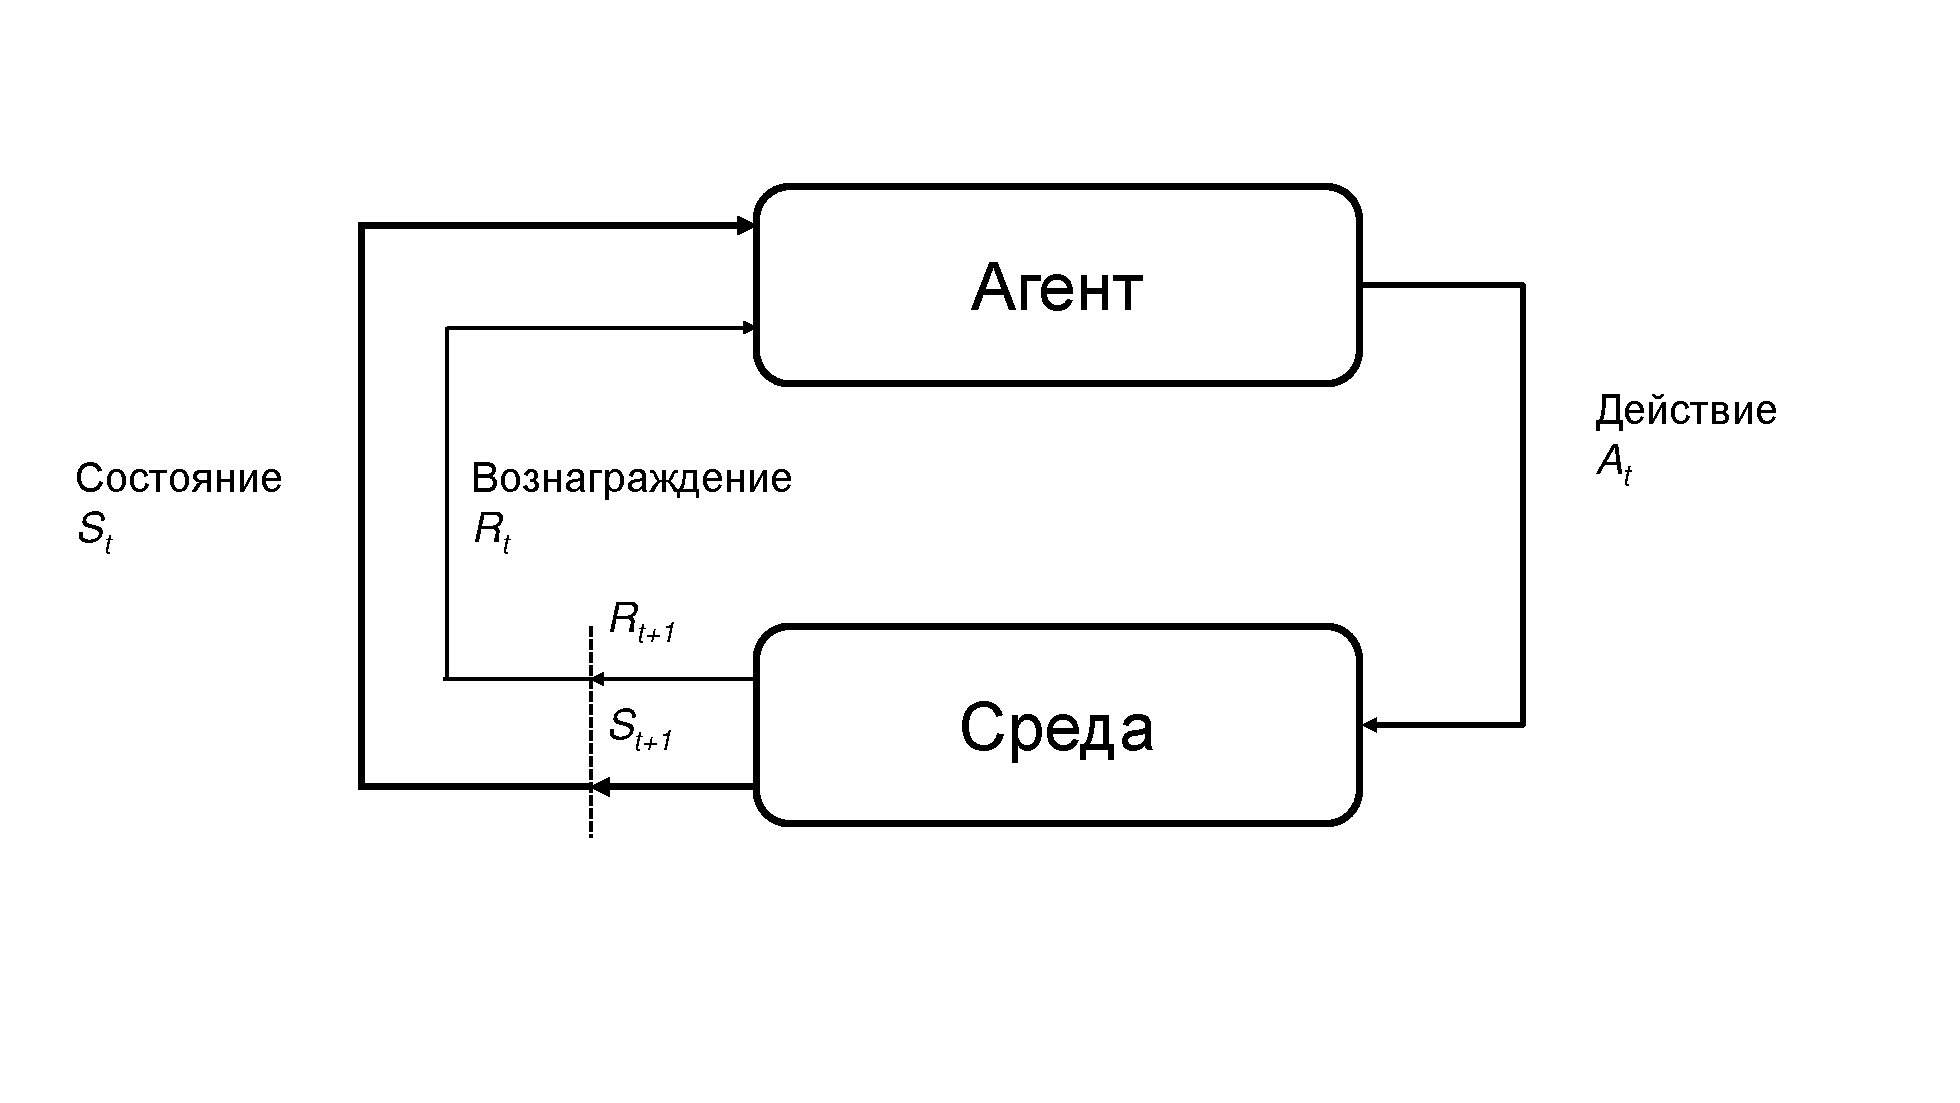
\includegraphics[scale = 0.4]{SARSA.pdf}}
	\caption{SARSA-модель}
\end{figure}

В англоязычной литературе данный процесс носит название «SARSA» («State-Action-Reward-State-Action-...»).\\

Вводится некоторая политика (англ. \textit{policy}):
\begin{center}
	$\pi \, : \; S \times A \rightarrow [0, 1]$

$\pi(a\,|\,s) = P(a_t=a\,|\,s_t=s)$ - вероятность действия $a$ в состоянии $s$.
\end{center}

Цель агента - выбрать такую оптимальную политику $\pi$, обозначающую вероятность выбора действия $a$ в состоянии $s$, чтобы при следовании ей сумма вознаграждений, получаемых от среды, была максимальна.
Ожидаемая награда в момент времени $t$ определяется как:

$$R_t = E[r_t \,+\, \gamma r_{t+1} \,+\, \gamma^2 r_{t+2}\, +\,\, ...] = E\left[\sum_{k=0}^{\infty}\gamma^kr_{t+k}\right],$$

где $E[\cdot]$ - математическое ожидание, $\gamma\in(0, 1)$ - коэффициент дисконтирования (англ. \textit{discount rate}).

Долгосрочная стратегия агента в общем случае не подразумевает преследование максимальной выгоды на каждом ромежуточном шаге. Непосредственный выбор стратегии может осуществляться множеством способов.
Введем функцию $Q(s,a)$ , которая парам состояние-действие ставит в соотвествие число. Данное число называется ценностью состояния-действия. Также на каждом временном шаге $ t $ агент получает вознаграждение $ r_{t} $:

$$Q^{\pi}(s, a) = E_{\pi}[R_t|\,s_t=s, a_t=a] = E_{\pi}\left[\sum_{k=0}^{\infty}\gamma^kr_{t+k}\,|\,s_t=s, a_t=a\right],$$

где индекс $\pi$ означает выбор действий в соотвествии с некоторой политикой (\textit{policy}).\\

Эта функция характеризует ожидаемую награду, получаемую агентом стартуя из состояния $s, s \in S$ совершая действие $a, a \in A$, и в дальнейшем действуя в соответсвии с определенной политикой $\pi$.

Отсюда мы можем получить рекурсивную формулу для оценки данной функции:\\

\begin{center}
	$Q_{i+1}^{\pi}(s, a) = E_{\pi}\left[r_t + \gamma\sum_{k=0}^{\infty}\gamma^kr_{t+k+1}\,|\,s_t=s, a_t=a\right] = E_{\pi}\left[r_t + \gamma Q_{i}^{\pi}(s_{t+1}=s', a_{t+1}=a')\,|\,s_t=s, a_t=a\right]$
\end{center}

Однако целью агента является - нахождение оптимальной политики $\pi$, на которой достигается максимальная ожидаемая награда. Таким образом, мы должны найти такую $\pi^*$, которая в результате нам дает максимальное значение action-value функции $Q^*(s, a)$ среди всех существующих политик. Формула для оценки оптимального значения action-value функции определяется следующим образом:
$$Q_{i+1}(s, a) = E[r_t + \gamma max_{a'}Q_i(s', a')\,|\,s, a]$$

При $i \rightarrow \infty$ следует, что $Q_{i}(s, a) \rightarrow Q^*(s, a)$. Данный процесс называется \textit{алгоритмом итерации значений} (англ. \textit{value iteration algorithm}).

\newpage
\begin{center}
\section{Постановка задачи}
\end{center}

\begin{figure}[H]
	{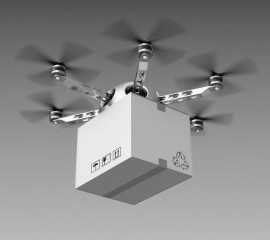
\includegraphics[scale = 0.6]{dronebw.jpg}}
	\caption{Беспилотный аппарат}
\end{figure}

Рассмотрим движение беспилотного аппарата (агента) в атмосфере (испытательной среде, лабиринте). Задачей агента является сбор грузов в различных точках пространтва и их доставка до точек выгрузки с наименьшими затратами топлива.\\

Агент движется в трёхмерном пространстве, каждому слою атмосферы соотвествует одна координата по оси Z, кроме того, происходит движение в плоскости $Oxy$. Каждой точке пространства соотвествует определённое значение плотности атмосферы, от которой зависит расход топлива, требуемого для перемещения.\\

Множество действий, доступных агенту состоит из восьми элементов:
\begin{itemize}
  	\item \textit{move south} - увеличение координаты $y$ на 1 (движение на юг);
	\item \textit{move north} - уменьшение координаты $y$ на 1 (движение на север);
	\item \textit{move east} - увеличение координаты $x$ на 1 (движение на восток);
	\item \textit{move west} - уменьшение координаты $x$ на 1 (движение на запад);
	\item \textit{move up} - увеличение координаты $z$ на 1 (движение вверх);
	\item \textit{move down} - уменьшение координаты $z$ на 1 (движение вниз);
	\item \textit{pickup} - сбор объекта;
	\item \textit{dropoff} - сброс объекта.	
\end{itemize}


\newpage
\begin{center}
\section{Q-learning алгоритм}
\end{center}

Поставленную задачу необходимо формализовать для применения метода обучения с подкреплением. Агентом является беспилотный аппарат, атмосфера выполняет роль внешней среды, обучающей агента. Взаимодействие со средой происходит при каждом действии агента на протяжении заданного промежутка времени или до достижения терминального состояния. На каждом временном шаге $ t $ агент получает некоторое описание состояния окружающей среды $ s_{t} \in S$, где $ S $ — множество возможных состояний среды, и на основании этого описания выбирает действие, где $ A(s_{t}) $ — множество действий, возможных в состоянии $s_{t}$.

Наиболее популряным алгоритмом в обучении с подкреплением явлется Q-learning алгоритм (Watkins, 1989). Популярность алгоритма обусловлена его простотой и эффективностью.

Название функции «Q», которая возвращает вознаграждение, используемое для обеспечения подкрепления, обозначает «качество» (англ. quality) действия, предпринимаемого агентом в определенном состоянии. 

Алгоритм относится к классу TD (Temporal-Difference). В TD-методах процесс обучения основывается на опыте взаимодействия агента со средой без использования модели среды. Расчетные оценки состояний (в случае задачи управления состояний-действий) в TD-методах обновляются, основываясь на других полученных оценках, т.е. они самонастраиваются [3].

В простом случае, одношаговый Q-learning алгоритм определеяется следующим образом:
\begin{center}
    $
    Q(S_{t}, A_{t}) \leftarrow Q(S_{t}, A_{t}) + \alpha[R_{t+1} + \gamma \max_{a} Q(S_{t+1}, a) - Q(S_{t}, A_{t})],
    $
\end{center}
где $\alpha$, $\gamma$ - параметры Q-learning. R - вознаграждание. $\alpha$ - это темп обучения, а $\gamma$ - дисконтирующий множитель. Гамма определяет, какую мы хотим придать важность вознаграждениям, ождиюащим нас в перпективе [4].

Алгоритм выглядит следующим образом [4]:
\begin{itemize}
    \item Инициализация произвольного $Q(s,a)$ $\forall s \in S, a \in A(s)$,
    \item Повторение для каждого эпизода:
    \begin{itemize}
        \item Инициализация S
        \item Повторение для каждого эпизода:
        \begin{itemize}
            \item Выбор A из S, получение вознаграждения R, подсчет S'
            \item Вычисление Q(S,A) по формуле выше
            \item Переход к новому состоянию S'
        \end{itemize}
    \end{itemize}
\end{itemize}


\newpage
\begin{center}
\section{Программная реализация}
\end{center}

Основой для решения послужила библиотека Gym от OpenAI [5]. Библиотека содержала, рассмотренную мной задачу в упрощённом виде: обучение с подкреплением использовалось для оптимизации обработки заказов и движения такси в двумерной плоскости.\\
Несмотря на кажущуюся схожесть с задачей управления беспилотным аппаратом, требовалась серьёзная доработка существующего решения:
\begin{itemize}
\item Требовалось обощить задачу на случай движения в трёх измерениях;
\item Требовалось изменить постановку задачи так, чтобы добавить физический и прикладной смыслы.
 \end{itemize}

Обе задачи были выполнены.\\ 

Основные компоненты программной реализации:
\begin{itemize}
\item main.py - основной файл, в котором реализовано обучение агента с помощью Q-learning, заданы параметры обучения (количетсво эпизодов, максимальное количетсво шагов в эпизоде, параметры Q-learning и т.д.)
\item labyrinth.py - файл, в котором реализованы 'правила' взаимодействия агента со средой.
\item map\_generation.py - файл, который содержит необходимые функции для построения символьного поля среды, в которой будет происходить обучение агента.
\item discrete.py - вспомогательный файл, который был разработан OpenAI для обучения с подкреплением.
 \end{itemize}

Код каждого файла представлен в Приложении.
Теперь рассмотрим каждую часть более подробно.
\begin{center}
    \subsection{Создание среды}
\end{center}

Как отмечалось выше, программа была реализована с помощью библиотеки \textit{gym} от OpenAI, так же был использован пакет \textit{numpy} для более удобной работы с матрицами.

В моей задаче, среда - это параллелепипед, задаваемый тремя параметрами (длина, ширина, высота). Создание символьного поля производится в файле map\_generation.py (см. Приложение), в котором c помощью символов +, -, | и : формируется среда, а так же случайным образом расставляются пункты назначения для агента (R(ed), G(green), B(lue), Y(ellow)) (см. рисунок ниже).
\begin{figure}[H]
	\center{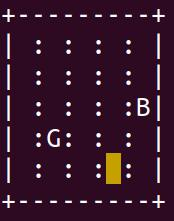
\includegraphics[scale = 0.70]{Location.jpg}}
	\caption{Слой в какой-то момент времени.}
\end{figure}

Основная цель данного символьного поля - провизуализировать перемещение агента в среде. Как отмечалось в разделе 'Постановка задачи', агенту доступны следующие действия (actions):
\begin{itemize}
\item Двигаться на юг (move south)
\item Двигаться на север (move north)
\item Двигаться на восток (move east)
\item Двигаться на запад (move west)
\item Двигаться наверх (move up)
\item Двигаться вниз (move down)
\item Подобрать объект (pickup)
\item Положить объект (dropoff)
 \end{itemize}

За каждое действие, агент получается очки (rewards). Они могут быть как очки вознаграждения, когда агент доставил объект из одной точки в другую, так и очки штрафы, когда агент сделал непраивльное действие, например, доставил объект не в то место или врезался в препятствие. Кроме того, за каждое перемещение агент теряет очки (топливо). И в зависимости от того, в какой ячейке находится агент, он затрачивает различное количество очков. За то, сколько необходимо потратить на перемещение отвечает функционал, который каждому набору данных в ячейке ставит в соответствие вознаграждение. В самом простом случае, в ячейке хранится уровень слоя, но в моей реализации среда также может учитывать плотность, давление и споротивление воздуха на данной высоте. При проведении различных испытаний, связанных с изменнием количества эпизодов обучения агента, параметров Q-learning и т.д. учитывается только высота слоя, поэтому вознаграждние рассчитывается следюущим образом:
\begin{center}
    reward = lay\_reward(lay),
\end{center}
где lay\_reward - это структура данных 'ключ-значение', где ключ - это номер слоя, а значение - очки на этом слое. В моём случае, нулевой слой соответсвует вознаграждению -(n+1)/2, а (n-1)-ый слой вознаграждению -1. Для более общего случая вводится трехмерный массив, который характирузует затраты топлива на перемещение в каждой точке слоя:
\begin{center}
    reward = cell\_reward[lay][row][column],
\end{center}
где, cell\_reward - трехмерный массив, а lay, row, column - это индексы для слоя, строки и столбца в этом массиве. Данная общая конструкция обеспечивает возможность ввести в модель сопротивление ветра, плотность и давление атмосферы.

Теперь рассмотрим количетсво возможных состояний в данной задаче. Всю среду можно представить в виде трехмерной сетки $size\_x \cdot size\_y \cdot size\_z$. Количетсво ячеек этой сетки равно количеству возможных расположений агента. В среде так же расположены 4 возможных места назначения. Если еще учесть одно состояние объекта: объект находится у агента, то можно подсчитать общее количество состояний в нашей среде для обучения агента. Итого, четыре возможных расположений пунктов назначений и 5 возможных расположений для объекта. Следовательно, в нашей среде насчитывается 
\begin{center}
    $N = size\_x \cdot size\_y \cdot size\_z \cdot 5 \cdot 4$
\end{center}
возможных состояний для агента. Агент взаимодейтсвует с одним из этих состояний и предпринимает решение, какое действие ему принять дальше.\\

После того, как было задано количество состояний, нужно учесть границы среды, чтобы в дальнейшем агент не смог за них выйти. Основную часть данного файла занимает шестивложенный цикл по следующим парметрам:
\begin{itemize}
    \item 3 пространственных параметра (lay, row, column)
    \item 2 по состояним объекта и пунктов назначения
    \item 1 по возможным действиям 
\end{itemize}
Внутри данного шестивложенного цикла происходит заполнение первичной таблицы вознаграждений под названием $P$. Данная таблица является матрицей, в котором количество столбцов соответсвует числу возможных действий, а количество строк соответствует количеству состояний. На рисунке ниже представлена данная матрица $P$ при рандомном индексе 442.
\begin{figure}[H]
	\center{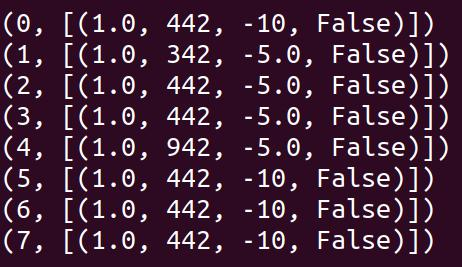
\includegraphics[scale = 0.70]{Actions_States.jpg}}
	\caption{P[442]}
\end{figure}
Как интерпретировать эти данные?
\begin{center}
    (action, [(probability, nextstate, reward, done)]),
\end{center}
Причем, 
\begin{itemize}
    \item значения 0 - 7 соответсвуют действиям (south, north, east, west, move up, move down, pickup, dropoff)
    \item done характеризует результат доставки объекта в пункт назначения
\end{itemize}
Каким же образом заполняется данная таблица? В шестивложенном цикле существует проверка на то, какое действие совершается и в зависимости от результата действия агент получает опредленное количество очков. Новое состояние получается при помощи функции encode и пяти параметров:
\begin{itemize}
    \item 3 пространственных (new\_lay, new\_row, new\_col)
    \item расположения объекта (new\_obj\_idx)
    \item расположения пункта назначения (desc\_idx)
\end{itemize}
В данном файле так же представлена функция render(), которая реализуют 2D-отрисовку перемещения агента в среде. В render используется decode(), которая преобразует входные данные в расположение агента, объекта и пунктов назначения при визуалиции. Ниже представлено несколько последовательных расположений агента в среде в виде куба со стороной 5:
\begin{figure}[H]
    \begin{minipage}[H]{0.24\linewidth}
        \center{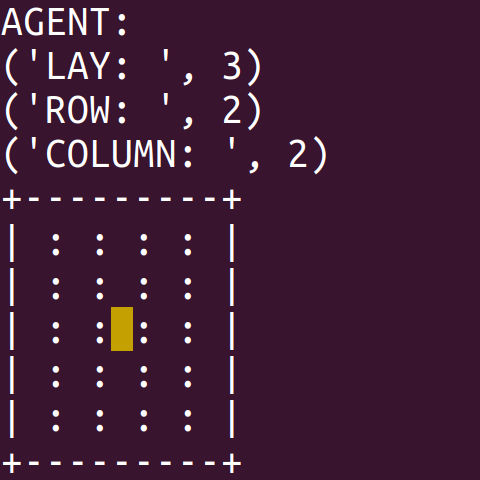
\includegraphics[width=1\linewidth]{0.png}} 0\\
    \end{minipage}
    \begin{minipage}[H]{0.24\linewidth}
        \center{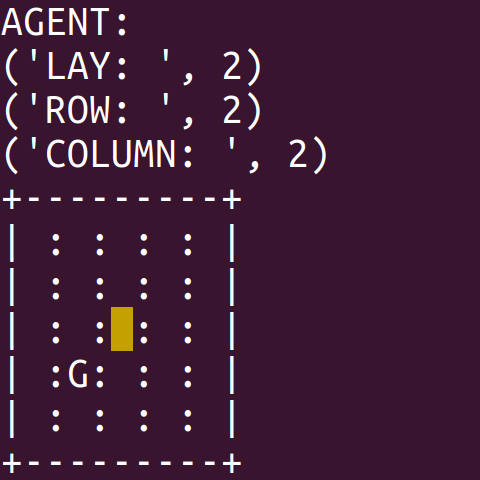
\includegraphics[width=1\linewidth]{1.png}} 1\\
    \end{minipage}
    \begin{minipage}[H]{0.24\linewidth}
        \center{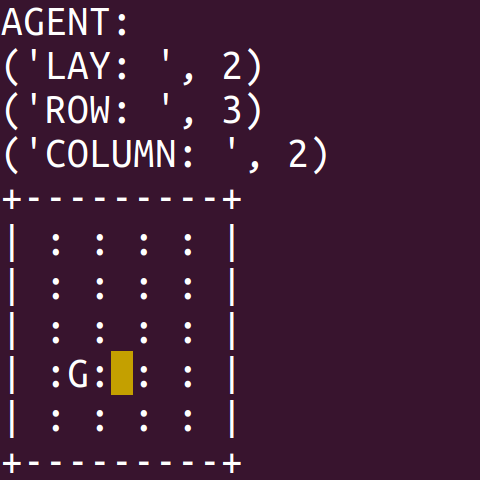
\includegraphics[width=1\linewidth]{2.png}} 2\\
    \end{minipage}
    \begin{minipage}[H]{0.24\linewidth}
        \center{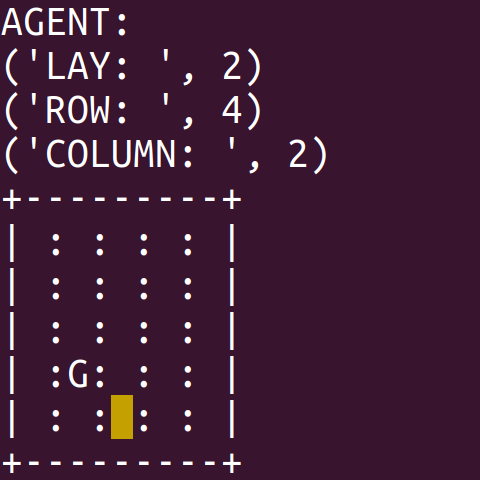
\includegraphics[width=1\linewidth]{3.png}} 3\\
    \end{minipage}
    \begin{minipage}[H]{0.24\linewidth}
        \center{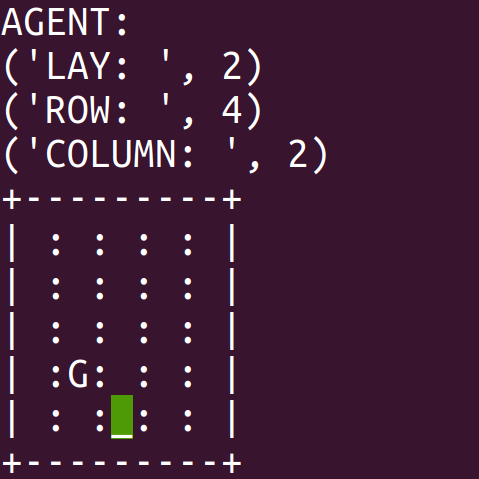
\includegraphics[width=1\linewidth]{4.png}} 4\\
    \end{minipage}
    \begin{minipage}[H]{0.24\linewidth}
        \center{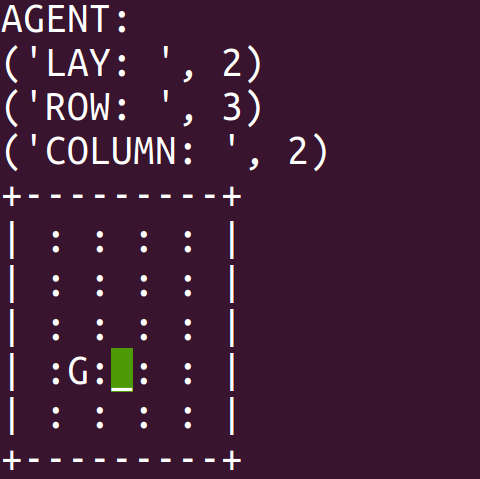
\includegraphics[width=1\linewidth]{5.png}} 5\\
    \end{minipage}
    \begin{minipage}[H]{0.24\linewidth}
        \center{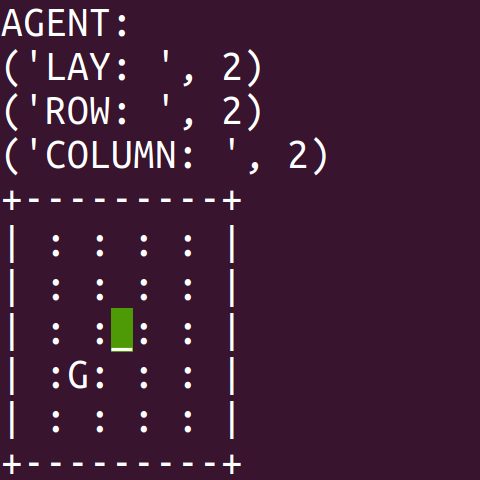
\includegraphics[width=1\linewidth]{6.png}} 6\\
    \end{minipage}
    \begin{minipage}[H]{0.24\linewidth}
        \center{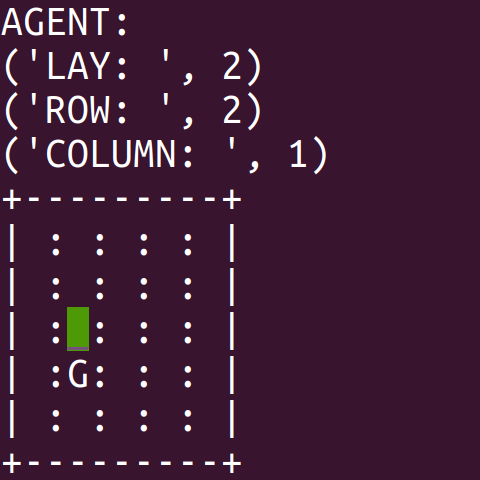
\includegraphics[width=1\linewidth]{7.png}} 7\\
    \end{minipage}
    \caption{Последовательность действий агента в одном из эпизодов}
    \label{fig:my_label}
\end{figure}
\\
Задача для агента формулируется следующим образом: "Доставить объект из пункта А в пункт Б с минимальными затратами топлива."
\begin{center}
    \subsection{Основной алгоритм: Q-learning}
\end{center}

Прежде всего, нужно заметить, что данную задачу можно решить другим способом без машинного обучения. С помощью цикла while можно написать алгоритм, который реализовывал бы доставку объекта и одной точки локации в другую, но, очевидно, что данный алгоритм был бы совершенно не эффективен на сетках любой размерности. Теперь перейдем к описанию самого алгоритма. \\

Используя среду, которую я описал в предыдущем подпункте и gym, я реализовал Q-learning алгоритм для поставленной задачи. Перед тем, как описывать реализацию алгоритма необходимо описать несколько полезных функций, которые были разработаны OpenAI. Прежде всего, env = gym.make() - это сердце OpenAI Gym, представляет собой интерфейс среды. У env есть несколько полезных методов:
\begin{itemize}
    \item env.step(action) - продвигает развитие оружающей среды на один шаг по времени.
    \item env.reset - обновляет среду, то есть перезапускает исходную среду и возвращает новое случайное исходное состояние.
\end{itemize}
Напомню основные детали Q-learning метода. Среда вознаграждает агента за постепенное обучение и за то, что в конкретном состоянии он совершает наиболее оптимальный шаг. В предыдущем подпункте я вводил таблицу $P$, по которой будет учиться агент. Опираясь на таблицу вознаграждений, он выбирает следующее действие в зависимости от того, насколько оно затратно, а затем обновляет величину, именуемую Q-значением. В результате создается новая таблица (Q-таблица), отображаемая на комбинацию (State, Action). Если Q-значения оказываются лучше, то получаются более оптимизированные вознаграждения. Например, если агент с объейктом находится в точке, в которой нужно выложить объект, то Q-значение для 'dropoff' оказывается выше, чем для остальных действий [6]. При взаимодейтсвии со средой Q-значение в Q-таблицы обновляется на основе следующей формулы:
\begin{center}
    $
    Q(s,a) = Q(s,a) + \alpha[R(s,a) + \gamma \max Q(s',a') - Q(s,a)],
    $
\end{center}
где $\alpha$, $\gamma$ - параметры Q-learning. R(s,a) - вознаграждание. $\alpha$ - это темп обучения, а $\gamma$ - дисконтирующий множитель. Гамма определяет, какую мы хотим придать важность вознаграждениям, ождиюащим нас в перпективе. Для того, чтобы агент был 'любопытным', вводится параметр $\epsilon$, отвечающий за так называемый exploration, то есть за исследование среды. Так же вводится параметр max\_steps, который отвечает за то, чтобы агент со временем перешел к следующему эпизоду, а не зашел в тупил из которого не может выйти.\\
\\
Сам алгоритм выглядит довольно просто:
\begin{enumerate}
    \item Инициализация Q-таблицы с нулями
    \item Цикл по количетсву эпизодов:
    \begin{enumerate}
        \item Перезапускаем среду (метод env.reset())
        \item Внутренни цикл по количеству максимальных шагов:
        \begin{enumerate}
            \item Взаимодействие агента со средой: выполнение доступных для агента действий в зависимости от 'любопытности' агента
            \item Переход к новому состоянию по результатам взаимодейтсвия со средой
            \item Обновление значений Q-таблицы по формуле, которая была представлена выше
            \item Новое состояние становится текущем состоянием
            \item Если агент не выполнин поставленную задачу, то алгоритм повторяется с п.(i)
            \item Если выполнин, то уменьшаем 'любопытность' агента и начинаем новый эпизод с п.(a)
        \end{enumerate}
    \end{enumerate}
\end{enumerate}

Дальше в файле main.py представлено обучение агента еще в нескольких эпизодах. Это было сделано для того, чтобы провизаулизировать как ведет себя агент при взаимодействии со средой.
\begin{center}
    \subsection{Вспомогательный файл от OpenAI}
\end{center}
Данный файл содержит необходимые для обучения агента методы, такие как:
\begin{itemize}
    \item reset() - перезапускает среду
    \item step() - продвигает развитие окружающей среды на один шаг
\end{itemize}

\newpage
\begin{center}
\section{Исследование поведения алгоритма}
\end{center}

Проведем ряд экспериментов над нашим алгоритмом. Будем варьировать количество эпизодов обучения, условия Q-learning'a (темп обучения $\alpha$ и дисконтирующий множитель $\gamma$), модель среды (учет высоты, плотность и давление воздуха, сопротивление ветра) и проанализируем полученные результаты.
\\
\begin{center}
    \subsection{Алгоритм без учета высоты, сопротивления ветра, давления и плотности воздуха}
\end{center}

Для начала рассмотрим как ведет себя алгоритм при $\alpha$ = 0 (темп обучения), $\gamma$ = 0.75 (дисконтирующий множитель, выбрали какое-то случайное значение), $\epsilon$ = 1 ('любопытность'  агента, которое изменяется в процессе обучения). Так же, зафиксируем нашу среду как куб со сторой равной 5. И будем варьировать количество эпизодов обучения N (total\_episodes). Рассмотрим следующие знчения N: 50, 500, 500, 5000. На графиках будет предсталвено две зависимоти: 1) Полученные экспериментальные точки. 2) Линейная аппроксимация этих точек для более информативного представления. 

\begin{figure}[H]
    \begin{minipage}[H]{0.49\linewidth}
       \center{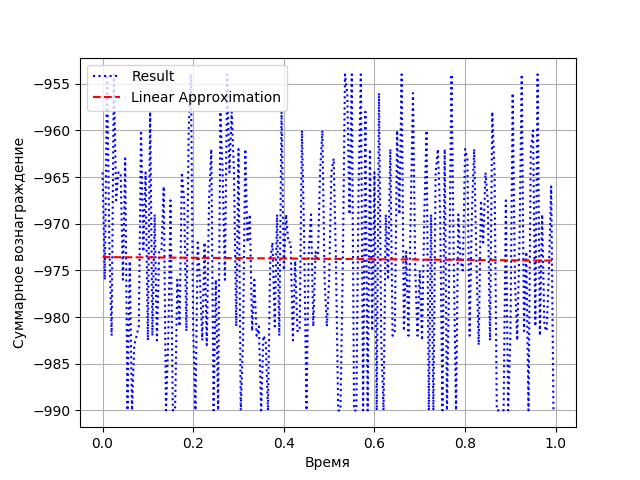
\includegraphics[width=1\linewidth]{withoutlayreward0_N50.png}} (a)\\
    \end{minipage}
    \hfill
    \begin{minipage}[H]{0.49\linewidth}
       \center{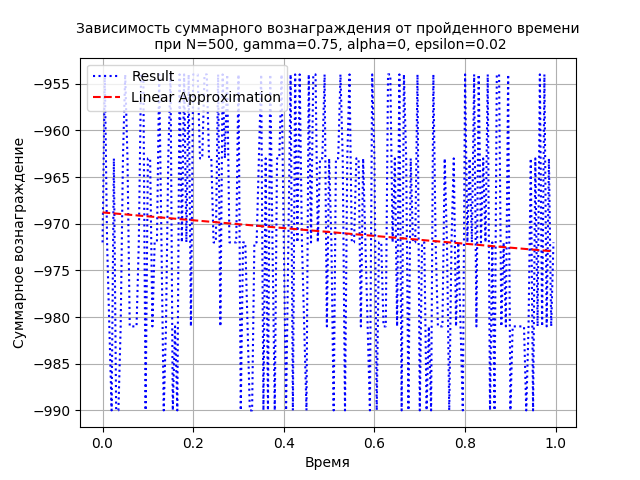
\includegraphics[width=1\linewidth]{withoutlayreward0_N500.png}} (б)\\
    \end{minipage}
    \caption{Зависимость суммарного вознаграждения от пройденного времени при $\alpha$=0, $\gamma$=0.75 и: (a) N=50; (б) N=500}
\end{figure}

\begin{figure}[H]
    \begin{minipage}[H]{0.49\linewidth}
       \center{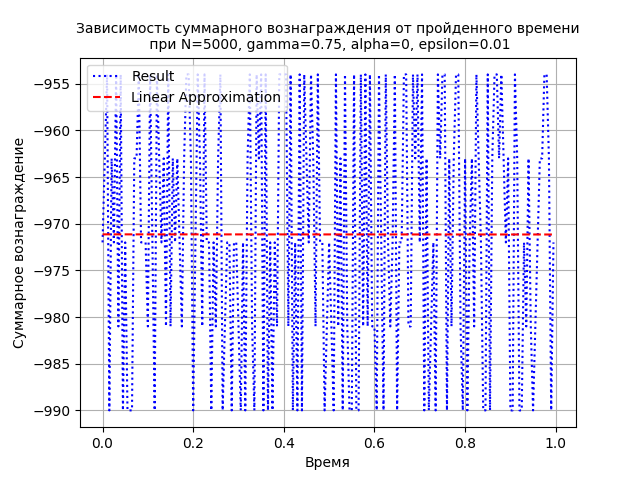
\includegraphics[width=1\linewidth]{withoutlayreward0_N5000.png}} (а)\\
    \end{minipage}
    \hfill
    \begin{minipage}[H]{0.49\linewidth}
       \center{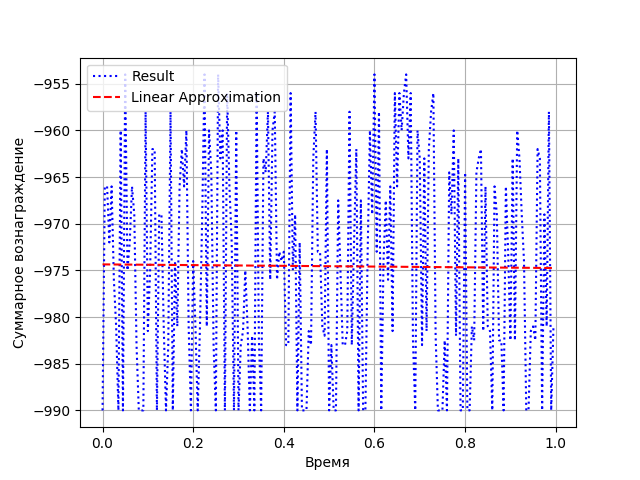
\includegraphics[width=1\linewidth]{withoutlayreward0_N50000.png}} (б)\\
    \end{minipage}
    \caption{Зависимость суммарного вознаграждения от пройденного времени при $\alpha$=0, $\gamma$=0.75 и: (a) N=5000; (б) N=50000}
\end{figure}

Получены достаточно ожидаемые графики. При нулевом темпе обучения, обучение агента практически не происходит и даже увеличение числа эпизодов обучения не дает адекватный результат. Поэтому, зафиксируем N=5000, оставим все остальные параметры с прежними значениями и проведем эксперименты с $\alpha$, изменяющимся с шагом 0.2.

\begin{figure}[H]
    \begin{minipage}[H]{0.49\linewidth}
       \center{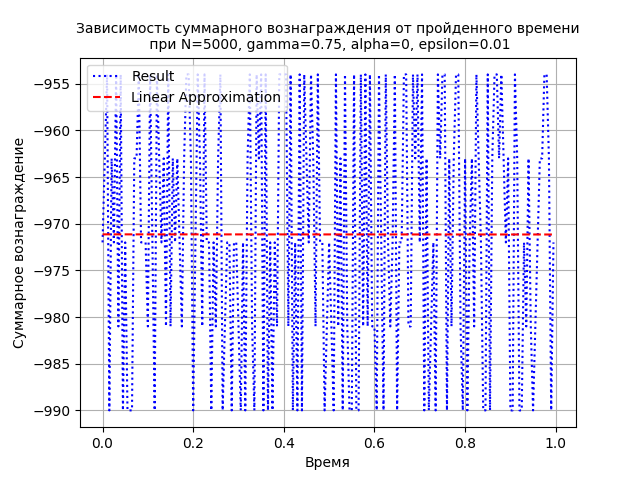
\includegraphics[width=1\linewidth]{withoutlayreward0_N5000.png}} (а)\\
    \end{minipage}
    \hfill
    \begin{minipage}[H]{0.49\linewidth}
       \center{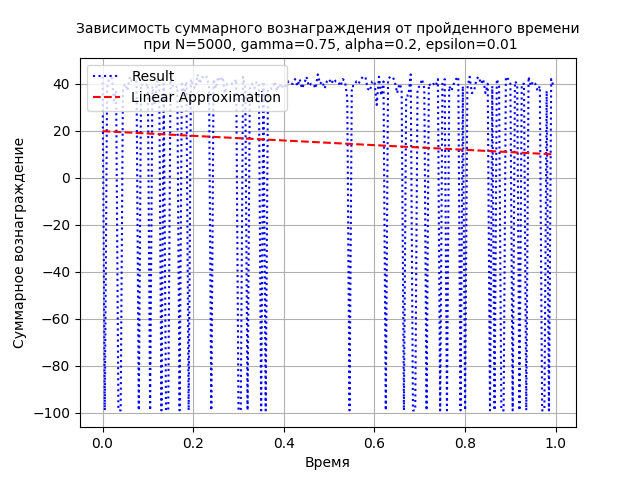
\includegraphics[width=1\linewidth]{withoutlayreward1_alpha0,2.png}} (б)\\
    \end{minipage}
      \caption{Зависимость суммарного вознаграждения от пройденного времени при N=5000, $\gamma$=0.75 и: (a) $\alpha$=0; (б) $\alpha$=0.2}
\end{figure}

\begin{figure}[H]
    \begin{minipage}[H]{0.49\linewidth}
       \center{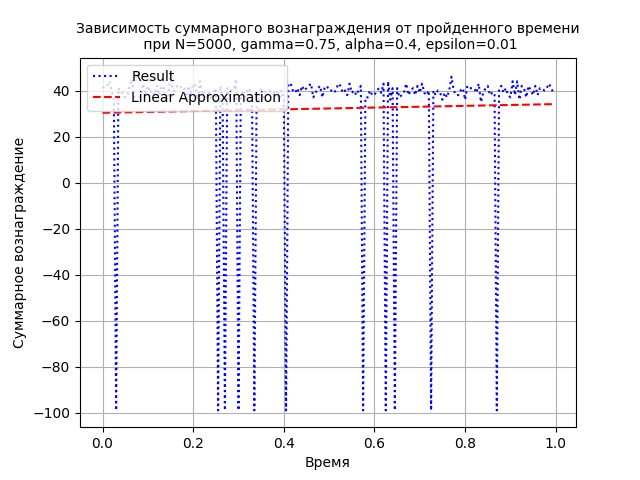
\includegraphics[width=1\linewidth]{withoutlayreward1_alpha0,4.png}} (а)\\
    \end{minipage}
    \hfill
    \begin{minipage}[H]{0.49\linewidth}
       \center{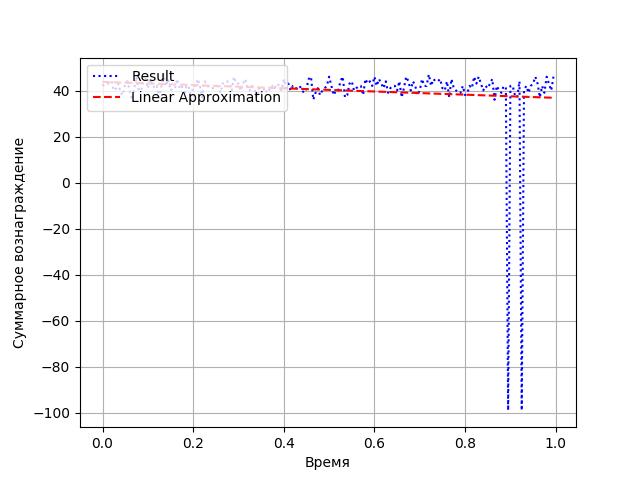
\includegraphics[width=1\linewidth]{withoutlayreward1_alpha0,6.png}} (б)\\
    \end{minipage}
    \caption{Зависимость суммарного вознаграждения от пройденного времени при N=5000, $\gamma$=0.75 и: (a) $\alpha$=0.4; (б) $\alpha$=0.6}
\end{figure}

\begin{figure}[H]
    \begin{minipage}[H]{0.49\linewidth}
       \center{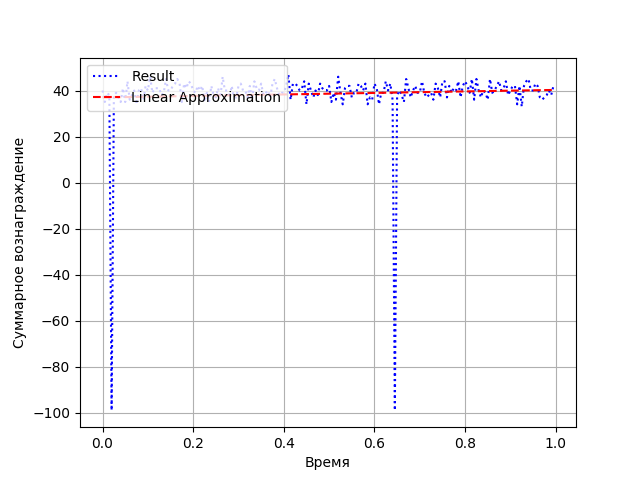
\includegraphics[width=1\linewidth]{withoutlayreward1_alpha0,8.png}} (а)\\
    \end{minipage}
    \hfill
    \begin{minipage}[H]{0.49\linewidth}
       \center{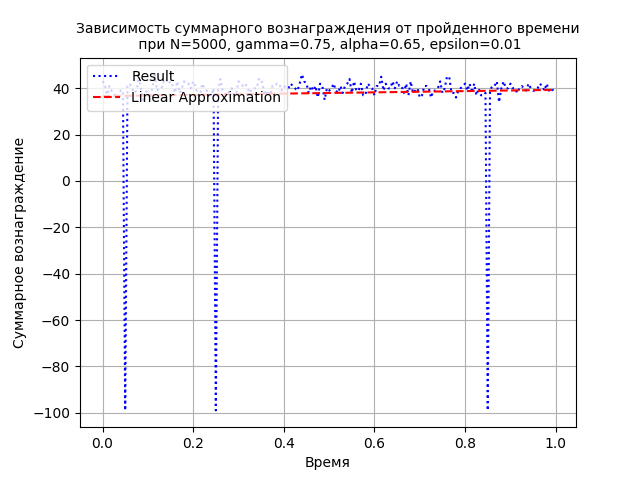
\includegraphics[width=1\linewidth]{withoutlayreward1_alpha1.png}} (б)\\
    \end{minipage}
    \caption{Зависимость суммарного вознаграждения от пройденного времени при N=5000, $\gamma$=0.75 и: (a) $\alpha$=0.8; (б) $\alpha$=1.0}
\end{figure}
\\
Как можно видеть из графиков, даже при N=5000, и $\alpha$ = 0.2 результат стал намного лучше: вознаграждание возрасло до 20-40, а при $\alpha$ = 0, оно было равно $\sim$(-1000). При увеличении параметра $\alpha$ до 1.0, можно наблюдать, что в какой-то момент при $\alpha$>0.6, получаемое вознаграждение получаемое агентом вышло на постоянное значение ($\sim$39). Следовательно, существует такое значение $\alpha$, при котором оно уже не будет вносить вклад в обучение, как бы его не увеличили. Проводя эксперимент при данных параметрах, я получил что точка насыщения для $\alpha$, т.е. при котором происходит выход на постоянное значение, равняется 0.63.
\\
Зафиксируем $\alpha$=0.63 и N=5000 и будем варьировать дисконтирующий множитель $\gamma$. Напомню, что данный параметр отвечает за то, какую мы хотим придать важность вознаграждениям, ожидающим нас в перспективе.
\begin{figure}[H]
    \begin{minipage}[H]{0.49\linewidth}
       \center{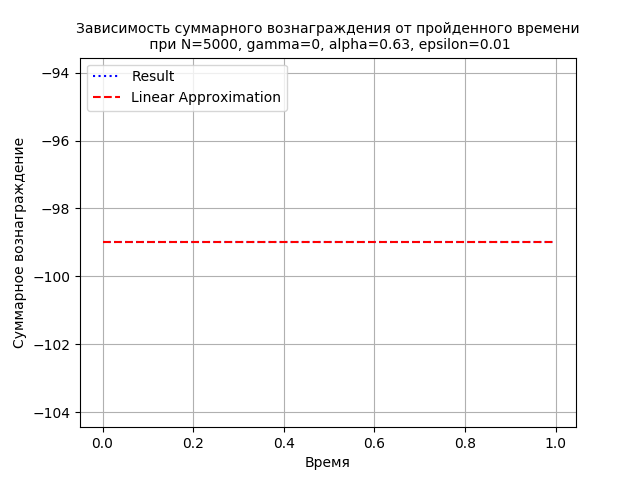
\includegraphics[width=1\linewidth]{withoutlayreward2_gamma0.png}} (а)\\
    \end{minipage}
    \hfill
    \begin{minipage}[H]{0.49\linewidth}
       \center{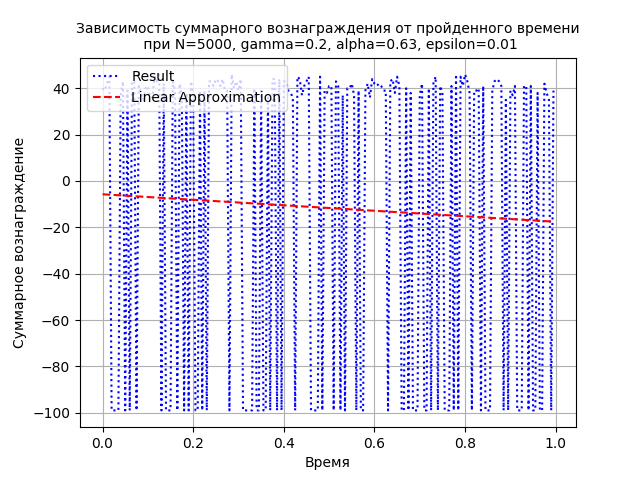
\includegraphics[width=1\linewidth]{withoutlayreward2_gamma0,2.png}} (б)\\
    \end{minipage}
    \caption{Зависимость суммарного вознаграждения от пройденного времени при N=5000, $\alpha$=0.63 и: (a) $\gamma$=0; (б) $\gamma$=0.2}
\end{figure}

\begin{figure}[H]
    \begin{minipage}[H]{0.49\linewidth}
       \center{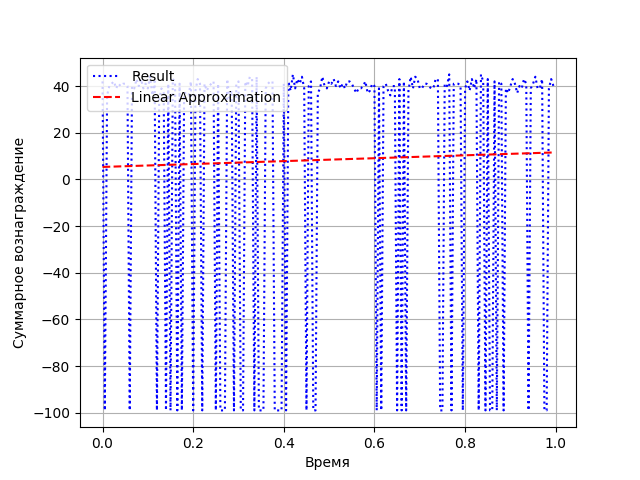
\includegraphics[width=1\linewidth]{withoutlayreward2_gamma0,4.png}} (а)\\
    \end{minipage}
    \hfill
    \begin{minipage}[H]{0.49\linewidth}
       \center{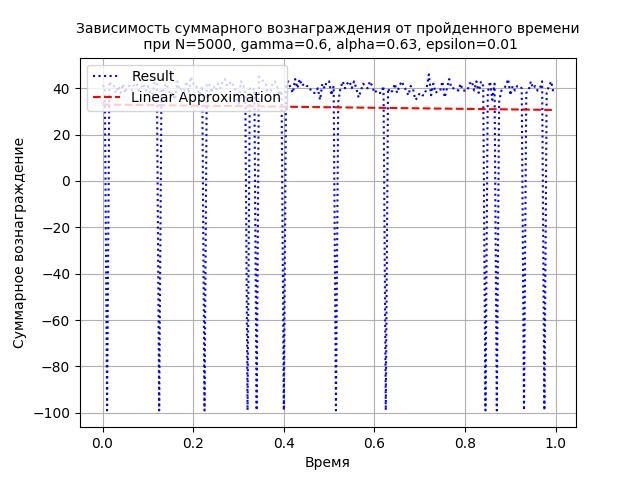
\includegraphics[width=1\linewidth]{withoutlayreward2_gamma0,6.png}} (б)\\
    \end{minipage}
     \caption{Зависимость суммарного вознаграждения от пройденного времени при N=5000, $\alpha$=0.63 и: (a) $\gamma$=0.4; (б) $\gamma$=0.6}
\end{figure}

\begin{figure}[H]
    \begin{minipage}[H]{0.49\linewidth}
       \center{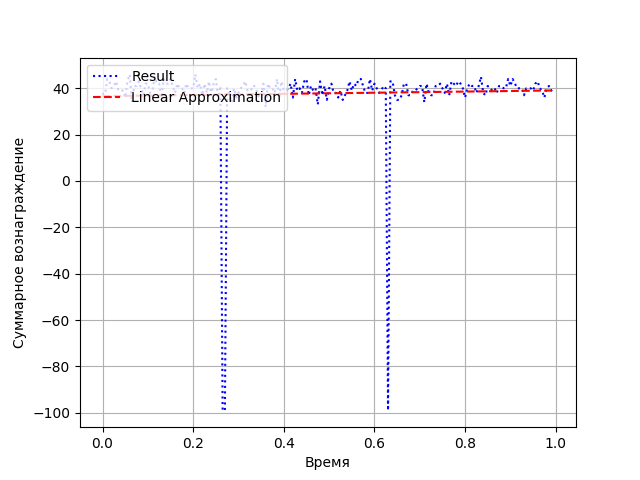
\includegraphics[width=1\linewidth]{withoutlayreward2_gamma0,8.png}} (а)\\
    \end{minipage}
    \hfill
    \begin{minipage}[H]{0.49\linewidth}
       \center{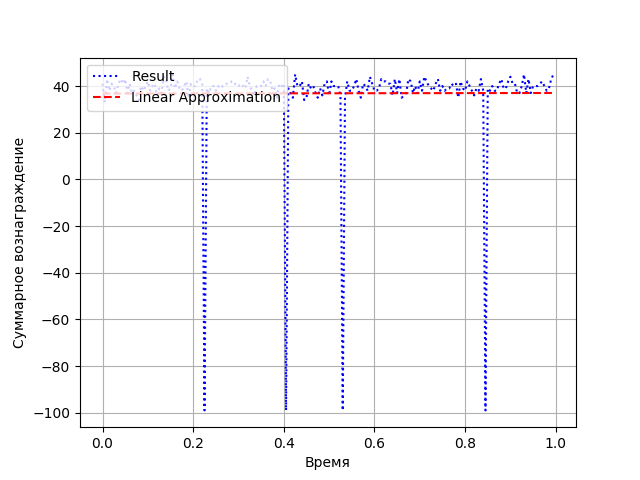
\includegraphics[width=1\linewidth]{withoutlayreward2_gamma1,0.png}} (б)\\
    \end{minipage}
     \caption{Зависимость суммарного вознаграждения от пройденного времени при N=5000, $\alpha$=0.63 и: (a) $\gamma$=0.8; (б) $\gamma$=1.0}
\end{figure}
\\
Как можно заметить из приведенных графиков, при $\gamma$=0 алгоритм ведет себя неадектано, но при увелечении $\gamma$, система достигает какого-то насыщения, т.е. существует такое значение параметра $\gamma$, при котором дальнейшнее увелечение данного параметра не дает вклада в обучение. Проводя ряд испытаний, я получил что оптимальное значение для $\gamma$ равняется 0.74 .
\\
\\
Также, хотелось бы привести примеры графиков, при значения $\alpha_{cr}$ = 1.45, $\gamma$ = 0.74 и $\gamma_{cr}$ = 1.05, $\alpha$ = 0.63. То есть, при таких параметрах, при которых происходят заметные ухудшения при обучении.
\begin{figure}[H]
    \begin{minipage}[H]{0.49\linewidth}
       \center{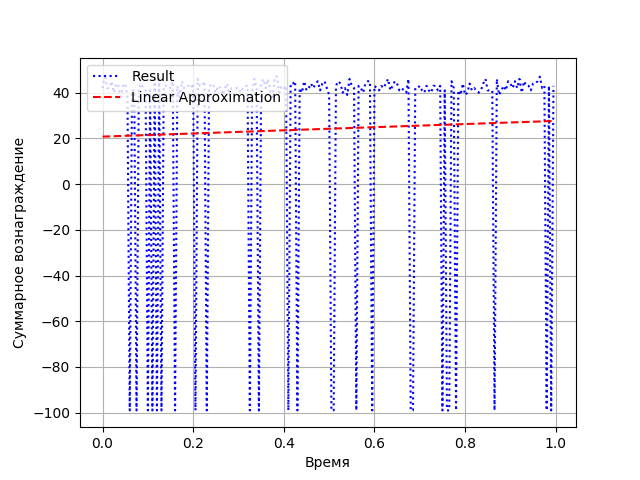
\includegraphics[width=1\linewidth]{withoutlayreward_critgamma.png}} (а)\\
    \end{minipage}
    \hfill
    \begin{minipage}[H]{0.49\linewidth}
       \center{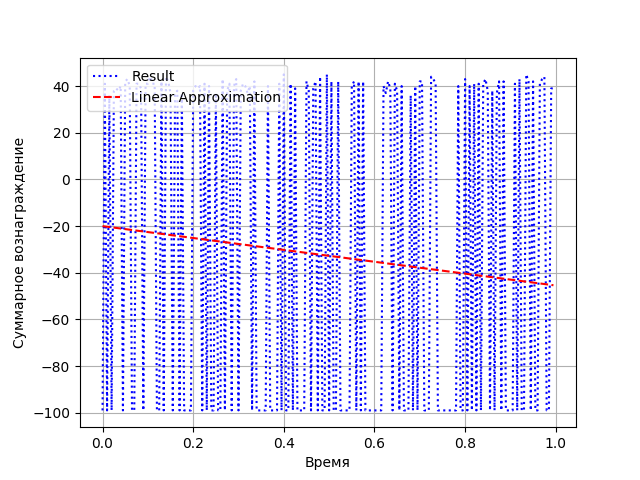
\includegraphics[width=1\linewidth]{withoutlayreward_critalpha.png}} (б)\\
    \end{minipage}
     \caption{Зависимость суммарного вознаграждения от пройденного времени при N=5000 и: (a) $\gamma_{cr}$=1.05, $\alpha$=0.63; (б) $\gamma$=0.74, $\alpha_{cr}$=1.45}
\end{figure}
Как можно заметить, при данных значениях параметров, обучение ведет себя сильно хуже.
\\
\begin{center}
    \subsection{Алгоритм с учетом высоты слоя}
\end{center}

В предыдущем пункте, была расссмотрена работа алгоритма без учета высоты, т.е. не была учита разряженность атмосферы при увеличении слоя, что было грубым допущением. Попробуем усложнить модель (в данном случае среду). Добавим в грубом приближении, что с увеличением слоя, будет затрачено меньше топлива на перемещение по слою в плоскости $Oxy$. 

Как отмечалось выше, за вознаграждение на каждом слое в модели, в которой учитывается только высота слоя отвечает следующая конструкция:
\begin{center}
    reward = lay\_reward(lay),
\end{center}
где lay\_reward - это структура данных 'ключ-значение', где ключ - это номер слоя, а значение - очки на этом слое. В моём случае, нулевой слой соответсвует вознаграждению - (n+1)/2, а (n-1)-ый слой вознаграждению -1.
\\
В предыдущем пункте было показано, что происходит с алгоритмом, если параметр $\alpha$=0. Поэтому, сразу перейдем к рассмотрию случая при котором мы будем варьировать $\alpha$ при фиксированном N. Пусть $\gamma$=0.75, N=5000, а $\alpha$ изменяется в пределах от 0 до 1.0.

\begin{figure}[H]
    \begin{minipage}[H]{0.49\linewidth}
       \center{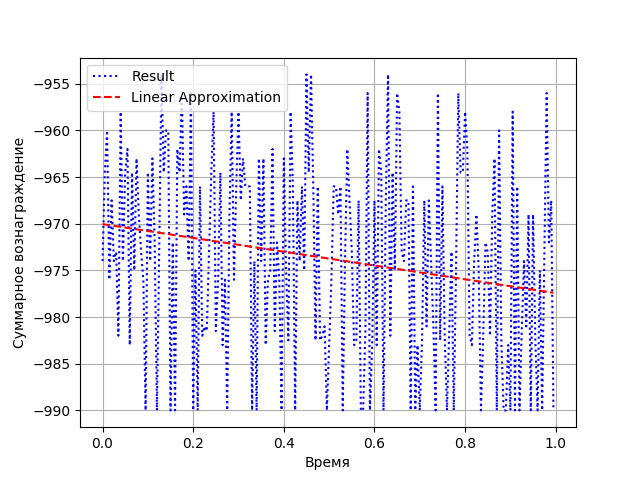
\includegraphics[width=1\linewidth]{reward_alpha_0.png}} (а)\\
    \end{minipage}
    \hfill
    \begin{minipage}[H]{0.49\linewidth}
       \center{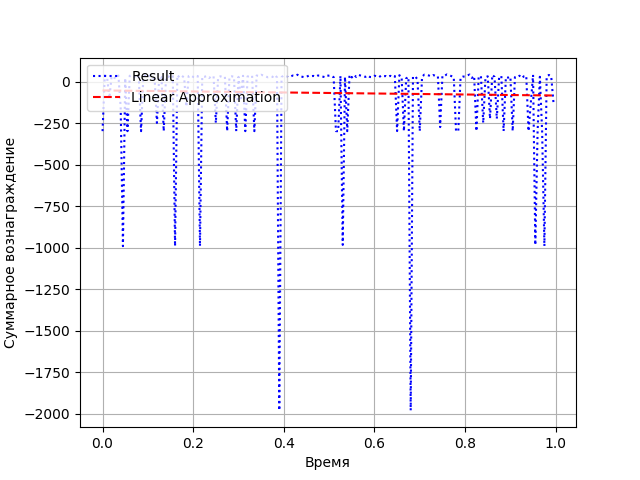
\includegraphics[width=1\linewidth]{reward_alpha_0,2.png}} (б)\\
    \end{minipage}
      \caption{Зависимость суммарного вознаграждения от пройденного времени при N=5000, $\gamma$=0.85 и: (a) $\alpha$=0; (б) $\alpha$=0.2}
\end{figure}
\begin{figure}[H]
    \begin{minipage}[H]{0.49\linewidth}
       \center{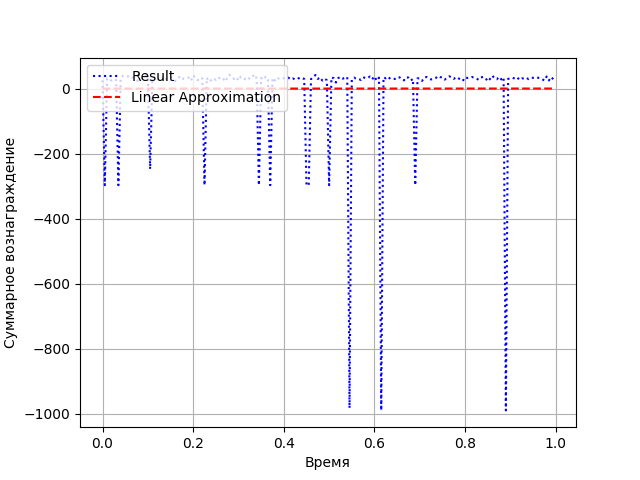
\includegraphics[width=1\linewidth]{reward_alpha_0,4.png}} (а)\\
    \end{minipage}
    \hfill
    \begin{minipage}[H]{0.49\linewidth}
       \center{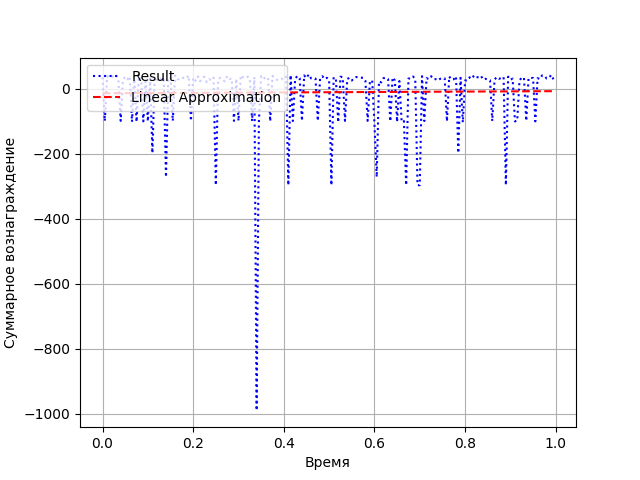
\includegraphics[width=1\linewidth]{reward_alpha_0,6.png}} (б)\\
    \end{minipage}
      \caption{Зависимость суммарного вознаграждения от пройденного времени при N=5000, $\gamma$=0.85 и: (a) $\alpha$=0.4; (б) $\alpha$=0.6}
\end{figure}
Из графиков выше, можно заметить, что аппроксимирующая зависимость лежит в зоне отрицательных значений вознаграждений. Можно задаться вопросом: "Адекватно ли работает алгоритм?". Да, алгоритм работает адекватно, так как важно смотреть не на то, сколько получает агент при обучении, а на то, улучшается ли тенденция при изменении параметров в 'нужную' сторону, если мы ожидаем увидеть там улучшение. Подбор нужных штрафов и вознаграждений довольно трудная задача, поэтому в данном эксперименте я больше ориетировался на тенденцию улучшения. Помимо увеличения $\alpha$, увеличим и N до 50000.
\begin{figure}[H]
    \begin{minipage}[H]{0.49\linewidth}
       \center{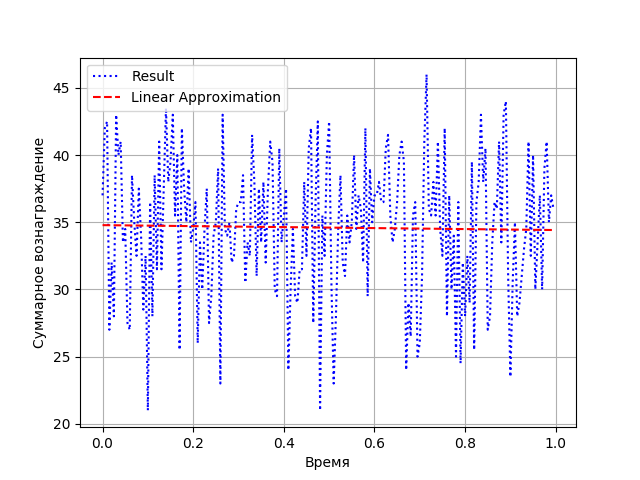
\includegraphics[width=1\linewidth]{reward1_alpha_0,4.png}} (а)\\
    \end{minipage}
    \hfill
    \begin{minipage}[H]{0.49\linewidth}
       \center{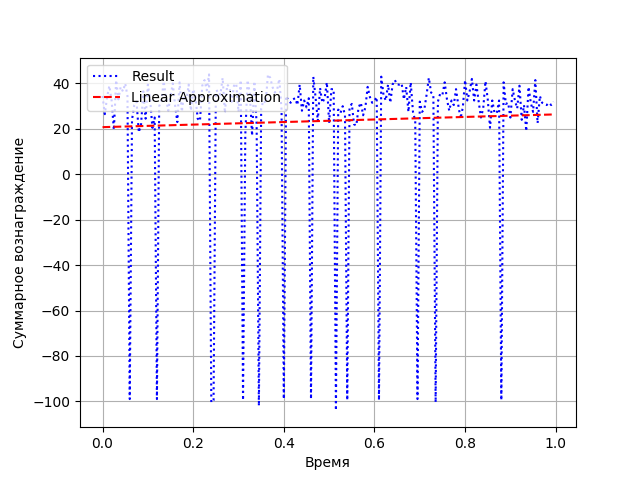
\includegraphics[width=1\linewidth]{reward1_alpha_0,6.png}} (б)\\
    \end{minipage}
      \caption{Зависимость суммарного вознаграждения от пройденного времени при N=50000, $\gamma$=0.85 и: (a) $\alpha$=0.4; (б) $\alpha$=0.6}
\end{figure}
Как можно заметить, улучшение произошло значительно, зависимость вышла из зоны отрициальных значений. Можно задаться вопросом: "Почему для данного алгоритма адекватный результат получился для N=50000, а в предыдщуем пункте насыщение произошло при N=5000?". Ответ на этот вопрос достаточно прост. Так как мы усложнили модель с помощью учета слоя, то агенту требуется больше времени на обучение. Поэтому, дальнейшие эксперименты будем проводить с N=50000.
\begin{figure}[H]
    \begin{minipage}[H]{0.49\linewidth}
       \center{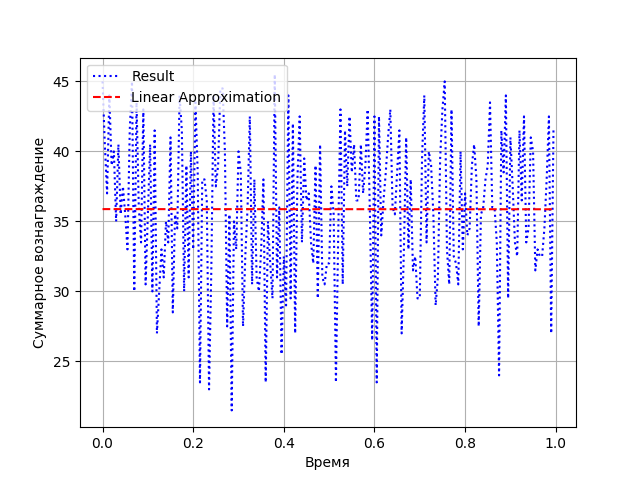
\includegraphics[width=1\linewidth]{reward1_alpha_0,8.png}} (а)\\
    \end{minipage}
    \hfill
    \begin{minipage}[H]{0.49\linewidth}
       \center{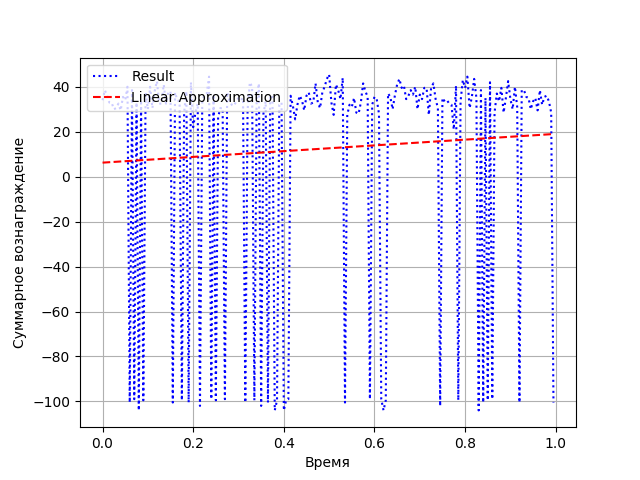
\includegraphics[width=1\linewidth]{reward1_alpha_1,0.png}} (б)\\
    \end{minipage}
      \caption{Зависимость суммарного вознаграждения от пройденного времени при N=50000, $\gamma$=0.85 и: (a) $\alpha$=0.8; (б) $\alpha$=1.0}
\end{figure}

Из приведенных графиков можно сделать вывод, что при увеличении $\alpha$ тенденция улучшается, но можно заметить, что при $\alpha$=1.0 зависимость выглядит хуже, чем для $\alpha$=0.8. Поэтому, необходимость пояснить, что алгоритм не всегда отрабаывает одинаково при каждом повторно запуске. Существуют отклонения, похожие на те, что продемострированы выше. Так как эта модель учитывает больше факторов, чем предыущая, то данные флуктуации требуют дополнительных исследований, но в данной работе я не буду останавливаться на этом и для дальнейшего обучения зафиксирую $\alpha$=0.77 (при данном параметры были получены адекватные результаты).

Теперь проведем ряд экспериментов с фикисированными $\alpha$=0.77 и N=50000. А варьировать будем $\gamma$.
\begin{figure}[H]
    \begin{minipage}[H]{0.49\linewidth}
       \center{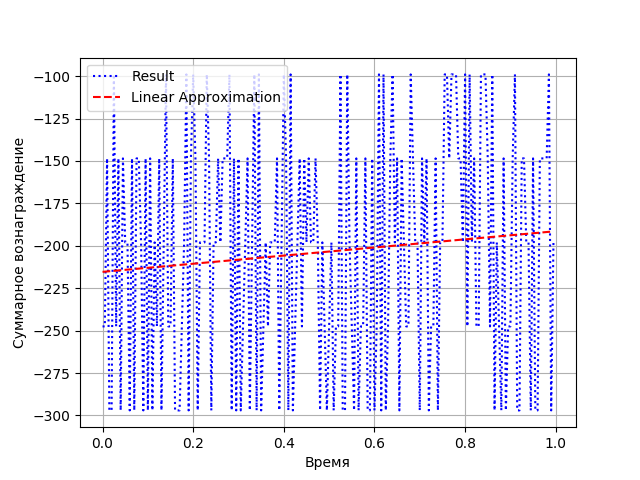
\includegraphics[width=1\linewidth]{reward_gamma_0.png}} (а)\\
    \end{minipage}
    \hfill
    \begin{minipage}[H]{0.49\linewidth}
       \center{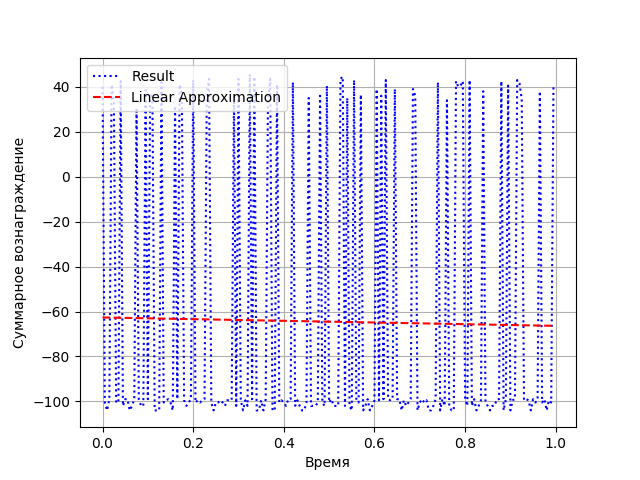
\includegraphics[width=1\linewidth]{reward_gamma_0,2.png}} (б)\\
    \end{minipage}
     \caption{Зависимость суммарного вознаграждения от пройденного времени при N=50000, $\alpha$=0.77 и: (a) $\gamma$=0; (б) $\gamma$=0.2}
\end{figure}
\begin{figure}[H]
    \begin{minipage}[H]{0.49\linewidth}
       \center{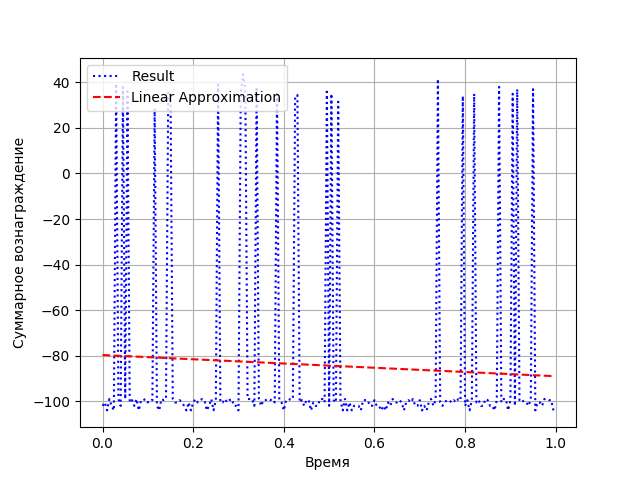
\includegraphics[width=1\linewidth]{reward_gamma_0,4.png}} (а)\\
    \end{minipage}
    \hfill
    \begin{minipage}[H]{0.49\linewidth}
       \center{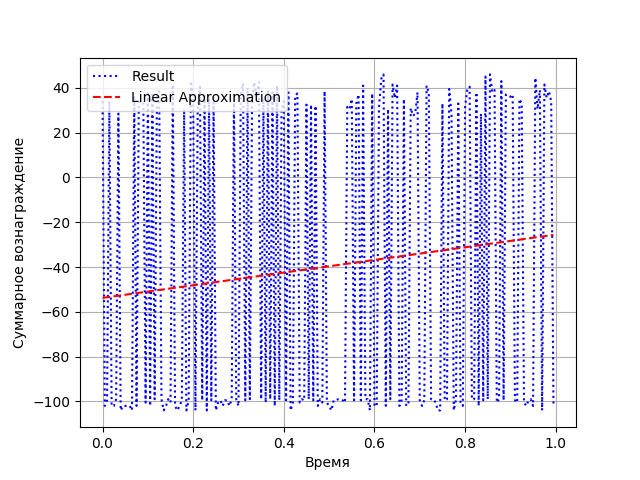
\includegraphics[width=1\linewidth]{reward_gamma_0,6.png}} (б)\\
    \end{minipage}
     \caption{Зависимость суммарного вознаграждения от пройденного времени при N=50000, $\alpha$=0.77 и: (a) $\gamma$=0.4; (б) $\gamma$=0.6}
\end{figure}
\begin{figure}[H]
    \begin{minipage}[H]{0.49\linewidth}
       \center{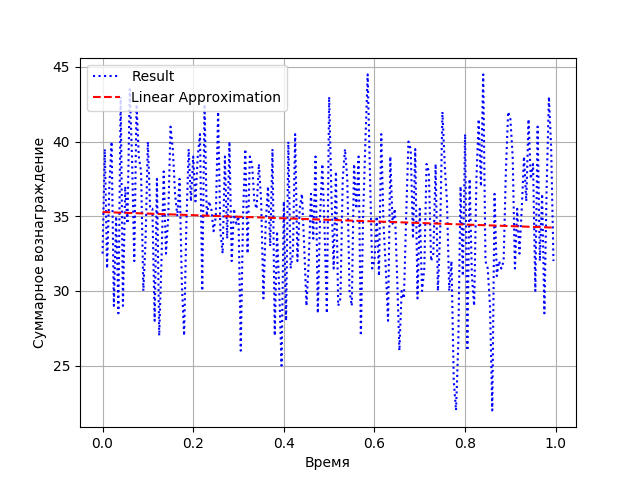
\includegraphics[width=1\linewidth]{reward_gamma_0,8.png}} (а)\\
    \end{minipage}
    \hfill
    \begin{minipage}[H]{0.49\linewidth}
       \center{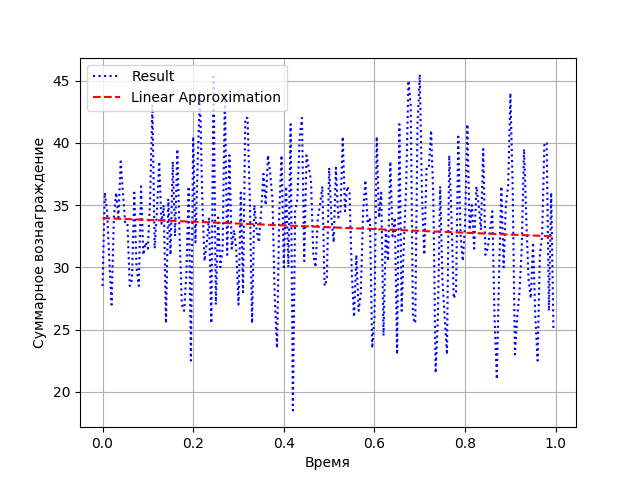
\includegraphics[width=1\linewidth]{reward_gamma_1,0.png}} (б)\\
    \end{minipage}
     \caption{Зависимость суммарного вознаграждения от пройденного времени при N=50000, $\alpha$=0.77 и: (a) $\gamma$=0.8; (б) $\gamma$=1.0}
\end{figure}

Можно заметить, что с увеличением $\gamma$, результаты при обучении получаются лучше с каждым разом. Но опять же, алгоритм выходит на насыщение. Оптимальный параметр $\gamma$ в данной модели равняется 0.86.

\begin{center}
    \subsection{Неудачные эксперименты}
\end{center}

При исследовании алгоритма, иногда попадались не совсем адекватные результаты эксперимента. Многое зависит от того, как ввести систему штрафов при обучении. Рассмотрим поведение алгоритма из пункта 6.2, если расход товлива на каждом слое вводится следующим образом: (а) нулевой слой соответсвует вознаграждению -n, а (n-1)-ый слой вознаграждению -1 (шаг 1 между слоями); (б) нулевой слой соответсвует вознаграждению -(n+1)/2, а (n-1)-ый слой вознаграждению -1 (шаг 0.5 между слоями). Представим два случая:
\begin{itemize}
    \item при оптимальном $\alpha$, N=50000 и чуть выше оптимального $\gamma$
    \item при оптимальном $\gamma$, N=50000 и чуть выше оптимального $\alpha$
\end{itemize}

\begin{figure}[H]
    \begin{minipage}[H]{0.49\linewidth}
       \center{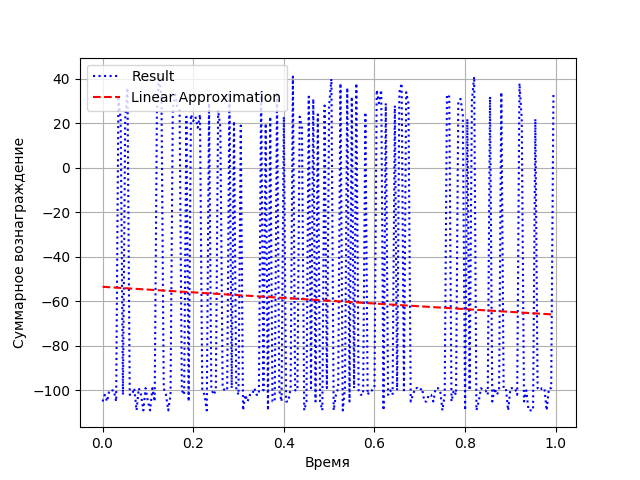
\includegraphics[width=1\linewidth]{bad_result.png}} (а)\\
    \end{minipage}
    \hfill
    \begin{minipage}[H]{0.49\linewidth}
       \center{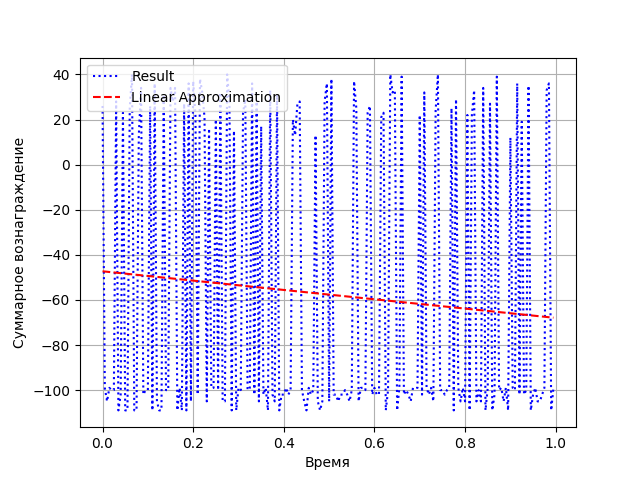
\includegraphics[width=1\linewidth]{nice_result.png}} (б)\\
    \end{minipage}
     \caption{Зависимость суммарного вознаграждения от пройденного времени при N=50000, $\alpha$=0.63, $\gamma$=0.8. (а) Случай при шаге 1. (б) Случай при шаге 0.5}
\end{figure}

\begin{figure}[H]
    \begin{minipage}[H]{0.49\linewidth}
       \center{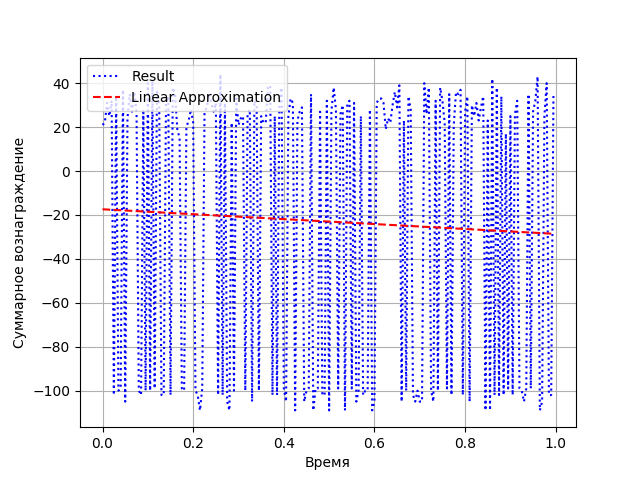
\includegraphics[width=1\linewidth]{bad_result_1.png}} (а)\\
    \end{minipage}
    \hfill
    \begin{minipage}[H]{0.49\linewidth}
       \center{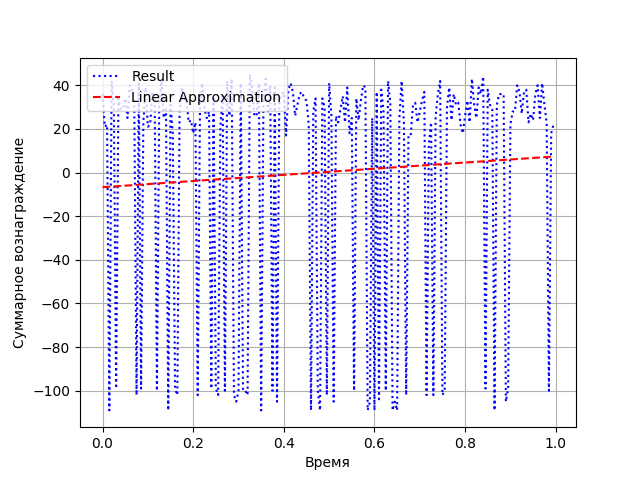
\includegraphics[width=1\linewidth]{nice_result_1.png}} (б)\\
    \end{minipage}
     \caption{Зависимость суммарного вознаграждения от пройденного времени при N=50000, $\alpha$=0.8, $\gamma$=0.73. (а) Случай при шаге 1. (б) Случай при шаге 0.5}
\end{figure}

Из графиков выше видно, что в случае (а) результаты заметно хуже. Если исследовать визуализацию алгоритма, то можно заметить почему это происходит. Агент стремится попасть попасть на самый разряженный слой (верхний), где затраты по топливу на перемещение минимальные. Как только он туда попадает он начинает перемещаться только по двум клеткам (агент заходит в тупик). Агент забывает о своей истинной цели и просто теряет очки.

\newpage
\begin{center}
    \section*{ЗАКЛЮЧЕНИЕ}
\end{center}
\addcontentsline{toc}{chapter}{ЗАКЛЮЧЕНИЕ}

В результате работы был разработан алгоритм для поиска пути в лабиринте. Задаче была поставлена в соответствие другая физическая задача - доставка дроном объектов из точки <А> в точку <Б>. Алгоритм был реализован на основе Q-learning. Были получены и интерпетированы графиик зависимостей суммарного вознаграждения агента при обучении в среде от времени обучения. На основе исследования алгоритма, были получены оптимальные параметры для обучения $\alpha$ (отвечает за темп обучения) и $\gamma$ (дисконтирующий множитель) в двух моделях:
\begin{itemize}
    \item Модель, в которой не учитываются физические параметры, такие как разряженнсость, давление, плотность и сопротивление воздуха.
    \item Модель, в котором учитывается разряженность воздуха.
\end{itemize}

Подводя итоги работы, можно сказать, что применение машинного обучения, нейронных сетей, в особенности Q-learning, в теории управления является одной из самых перспективных областей. В данной работе были наглядно продемонстрированы возможности искусственного интеллекта к самообучению, используя метод «проб и ошибок».

Дальнейшее развитие данной задачи выглядит весьма многообещающим:
\begin{itemize}
    \item Усложнить модель. Внести в неё более полный учет параметров воздуха, таких как давление, плотность и сопротивление.
    \item Реализовать алгоритм Deep Q-learning, который является более эффективным по сравнению с Q-learning.
    \item Реализовать метод сопряженных градиентов для более эффективного поиска параметров Q-learning.
    \item Использовать реальные физические данные атмосфер, которые бы преобразовывались с помощью функционала в пространство вознаграждений для агента.
     \item Реализовать 3D-визуализацию перемещения агента в среде, где будут отмечены области, в которых агенту перемещаться менее затратно, чем в других.
\end{itemize}

\newpage
\begin{center}
    \section*{СПИСОК ИСПОЛЬЗУЕМЫХ ИСТОЧНИКОВ} 
\end{center}
\addcontentsline{toc}{chapter}{СПИСОК ИСПОЛЬЗУЕМЫХ ИСТОЧНИКОВ}
$[1]$ - Сайт англоязычной википедии. Интернет ресурс: https://en.wikipedia.org/wiki/Machine\_learning
$[2]$ -  Саттон Р., Барто Э. Обучение с подкреплением – Бином. Лаборатория знаний,
2012. – 400 с.\\
$[3]$ - Князятов С.А., Малинецкий Г.Г.,
Решение задачи распознавания блефа в игре «верю – не верю» с помощью алгоритмов
обучения с подкреплением // Препринты ИПМ им. М.В.Келдыша. 2018. No 170. 21 с.\\
$[4]$ - Richard S. Sutton and Andrew G.Barto - Reinforcement Learning:
An Introduction \\
$[5]$ - Библиотека gym от OpenAi. Интернет ресурс: https://gym.openai.com \\
$[6]$ - Обучение с подкреплением на языке Python. Интернет ресурс: https://habr.com/ru/company/piter/blog/434738/


\newpage
\begin{center}
\section*{ПРИЛОЖЕНИЕ}
\end{center}

\addcontentsline{toc}{chapter}{ПРИЛОЖЕНИЕ}

\begin{lstlisting}[label=some-code, caption=labyrinth.py]
import sys
from contextlib import closing
from six import StringIO
import os
import time
from gym import utils
from gym.envs.toy_text import discrete
#from gym.envs.toy_text import map_generation as mg
import map_generation as mg
import numpy as np

x_size = 5
y_size = x_size
z_size = x_size

#functional that sets of paramenters in accordance with rewa
rd
def functional(inPut):
    out = 0
    for val in inPut:
        out += inPut[val]
    return out

lay_reward = {}
counter = -1
fine_step = 0.5
for a in range(z_size-1,-1,-1):
    lay_reward[a] = counter
    counter = counter - fine_step

cell_reward = np.zeros((x_size, y_size, z_size))
for z, lay in enumerate(cell_reward):
    struct = {
        'Lay Reward': lay_reward[z],
        'Density': 0,
        'Wind': 0,
        }
    for y, col in enumerate(lay):
        for x, row in enumerate(col):
            result = functional(struct)
            cell_reward[z][y][x] = result

taxi_map = mg.Map()
taxi_map.map_creation(x_size, y_size, z_size)
d = taxi_map.loc_creation()

colors = ['R', 'G', 'Y', 'B']

def get_minimum(new_location, limit):
    boom = False
    if new_location > limit:
        return limit, True
    return new_location, boom

def get_maximum(new_location, limit):
    boom = False
    if new_location < limit:
        return limit, True
    return new_location, boom
    
class TaxiEnv(discrete.DiscreteEnv):
    metadata = {'render.modes': ['human', 'ansi']}

    def __init__(self):
        self.desc = np.asarray(taxi_map.MAP, dtype='c')
        self.locs = []

        for c in colors:
            self.locs.append(d[c])

        num_states = taxi_map.volume()*5*4
        num_rows = y_size
        num_columns = x_size
        num_lays = z_size
        max_row = num_rows - 1
        max_col = num_columns - 1
        max_lay = num_lays - 1
        
        initial_state_distrib = np.zeros(num_states)
        num_actions = 8
        P = {state: {action: []
                     for action in range(num_actions)} for state in range(num_states)}
        # Running through layers (Z-axis)
        for lay in range(num_lays):
            # Running through rows (Y-axis)
            for row in range(num_rows):
                # Running through columns (X-axis)
                for col in range(num_columns):
                    # +1 for being inside taxi; below
                    for obj_idx in range(len(self.locs) + 1): 
                        for dest_idx in range(len(self.locs)):
                            state = self.encode(lay, row, col, obj_idx, dest_idx)
                            if obj_idx < 4 and obj_idx != dest_idx:
                                initial_state_distrib[state] += 1
                            for action in range(num_actions):
                                new_lay, new_row, new_col, new_obj_idx = lay, row, col, obj_idx
                                #reward = lay_reward[lay]
                                reward = cell_reward[lay][col][row]
                                done = False
                                taxi_loc = (lay, row, col)
                                # 0 - south
                                if action == 0:
                                    new_row, boom = get_minimum(row + 1, max_row)
                                    if boom:
                                        reward = -10
                                # 1 - north
                                elif action == 1:
                                    new_row, boom = get_maximum(row - 1, 0)
                                    if boom:
                                        reward = -10
                                # 2 - east
                                if action == 2 and self.desc[lay, 1 + row, 2 * col + 2] == b":":
                                    new_col, boom = get_minimum(col + 1, max_col)
                                    if boom:
                                        reward = -10
                                # 3 - west
                                elif action == 3 and self.desc[lay, 1 + row, 2 * col] == b":":
                                    new_col, boom = get_maximum(col - 1, 0)
                                    if boom:
                                        reward = -10
                                # 4 - move up
                                if action == 4:  # and self.desc[lay, 1 + row, 2 * col + 2] == b":":
                                    new_lay, boom = get_minimum(lay + 1, max_lay)
                                    if boom:
                                        reward = -10
                                # 5 - move down
                                elif action == 5:  # and self.desc[lay, 1 + row, 2 * col] == b":":
                                    new_lay, boom = get_maximum(lay - 1, 0)
                                    if boom:
                                        reward = -10
                                # 6 - pickup
                                elif action == 6:  # pickup
                                    if (obj_idx < 4) and (taxi_loc == self.locs[obj_idx]):
                                        new_obj_idx = 4
                                    else:  #object not at location
                                        reward = -10
                                # 7 - dropoff
                                elif action == 7:  # dropoff
                                    if (taxi_loc == self.locs[dest_idx]) and obj_idx == 4:
                                        new_obj_idx = dest_idx
                                        done = True
                                        reward = 50
                                    elif (taxi_loc in self.locs) and obj_idx == 4:
                                        new_obj_idx = self.locs.index(taxi_loc)
                                    else:  # dropoff at wrong location
                                        reward = -20
                                new_state = self.encode(
                                    new_lay, new_row, new_col, new_obj_idx, dest_idx)
                                P[state][action].append(
                                    (1.0, new_state, reward, done))
        initial_state_distrib /= initial_state_distrib.sum()
        discrete.DiscreteEnv.__init__(
            self, num_states, num_actions, P, initial_state_distrib)

    def encode(self, taxi_lay, taxi_row, taxi_col, obj_loc, dest_idx):
        i = taxi_lay
        i *= z_size
        i += taxi_row
        i *= y_size
        i += taxi_col
        i *= x_size
        i += obj_loc
        i *= 4
        i += dest_idx
        return i

    def decode(self, i):
        out = []
        out.append(i % 4)
        i = i // 4
        out.append(i % x_size)
        i = i // x_size
        out.append(i % y_size)
        i = i // y_size
        out.append(i % z_size)
        i = i // z_size
        out.append(i)
        assert 0 <= i < 5
        return reversed(out)

    def render(self, mode='human'):
        outfile = StringIO() if mode == 'ansi' else sys.stdout

        out = self.desc.copy().tolist()
        out = [[[c.decode('utf-8') for c in line] for line in lay] for lay in out]
        taxi_lay, taxi_row, taxi_col, obj_idx, dest_idx = self.decode(self.s)
        def ul(x): return "_" if x == " " else x
        if obj_idx < 4:
            out[taxi_lay + 1][1 + taxi_row][2 * taxi_col + 1] = utils.colorize(
                out[taxi_lay + 1][1 + taxi_row][2 * taxi_col + 1], 'yellow', highlight=True)
            pk, pj, pi = self.locs[obj_idx]
            out[pk + 1][pi + 1][2 * pj + 1] = utils.colorize(out[pk + 1][pi + 1][2 * pj + 1], 'blue', bold=True)
        else:  #agent with object
            out[taxi_lay + 1][1 + taxi_row][2 * taxi_col + 1] = utils.colorize(
                ul(out[taxi_lay + 1][1 + taxi_row][2 * taxi_col + 1]), 'green', highlight=True)

        dk, di, dj = self.locs[dest_idx]
        out[dk + 1][di + 1][2 * dj + 1] = utils.colorize(out[dk + 1][di + 1][2 * dj + 1], 'magenta')
        os.system('clear')
        print("AGENT:")
        print("LAY: ", taxi_lay)
        print("ROW: ", taxi_row)
        print("COLUMN: ", taxi_col)
        outfile.write("\n".join(["".join(row) for row in out[taxi_lay + 1]]) + "\n")
        time.sleep(5)
        #print all lays below
        #print("ALL LAYS")
        #for item in out:
        #   outfile.write("\n".join(["".join(row) for row in item]) + "\n")
        if self.lastaction is not None:
            outfile.write("  ({})\n".format(["South", "North", "East", "West", "MoveUp", "MoveDown", "Pickup", "Dropoff"][self.lastaction]))
        else:
            outfile.write("\n")
        if mode != 'human':
            with closing(outfile):
                return outfile.getvalue()

print('labyrinth.py launched successfully')
print('\n')
\end{lstlisting}

\begin{lstlisting}[label=some-code, caption=main.py]
import numpy as np
import scipy as sp
import gym
import random
import time
import os
import matplotlib
import matplotlib.pyplot as plt

env = gym.make("Taxi-v2")
env.render()

action_size = env.action_space.n
state_size = env.observation_space.n

qtable = np.zeros((state_size, action_size))

total_episodes = 50000        # Total episodes
total_test_episodes = 200     # Total test episodes
max_steps = 99                # Max steps per episode

#0 < ... <= 1
alpha = 0.63                  # Learning rate
gamma = 0.75                  # Discounting rate

# Exploration parameters
epsilon = 1.0                 # Exploration rate

max_epsilon = 1.0             # Exploration probability at s
tart
min_epsilon = 0.01            # Minimum exploration probabil
ity
decay_rate = 0.01

def plotting(action, step, done, info):
    print("ACTION: ", action)
    print("STEP: ", step)
    print("DONE: ", done)
    print("INFO: ", info)
    print("TOTAL REWARD: ", total_rewards)

score_ov_time =[]
x_steps = []
for episode in range(total_episodes):
    # Reset the environment
    state = env.reset()
    step = 0
    done = False
    
    for step in range(max_steps):
        #randomize a number
        exp_exp_tradeoff = random.uniform(0,1)
        
        #If this number > greater than epsilon --> exploitation
        #(taking the biggest Q value for this state)
        if exp_exp_tradeoff > epsilon:
            action = np.argmax(qtable[state,:])
        
        # Else doing a random choice --> exploration
        else:
            action = env.action_space.sample()
        
        #Take the action (a) and observe
        #the outcome state(s') and reward (r)
        new_state, reward, done, info = env.step(action)

        # Update Q(s,a):= Q(s,a) + alpha
        #[R(s,a) + gamma * max Q(s',a') - Q(s,a)]
        qtable[state, action] = qtable[state, action] + alpha*(reward + gamma * 
                                    np.max(qtable[new_state,:]) - qtable[state, action])
        #new state is state
        state = new_state
        
        # If done : finish
        if done == True: 
            break
    
    # Reduce epsilon
    epsilon = min_epsilon + (max_epsilon - min_epsilon)*np.exp(-decay_rate*episode)

env.reset()
rewards = []

for episode in range(total_test_episodes):
    state = env.reset()
    x_steps.append(episode / total_test_episodes)
    step = 0
    done = False
    total_rewards = 0
    #os.system("clc||clear")
    #print("*****************")
    #print("EPISODE: ", episode)
    for step in range(max_steps):
        #FOR VISUALIZATION
        #env.render()
        #Take the action (index) that have the maximum
        #expected future reward given that state
        action = np.argmax(qtable[state,:])
        new_state, reward, done, info = env.step(action)
        total_rewards += reward
        #plotting(action, step, done, info)
        if done:
            rewards.append(total_rewards)
            #print ("Score", total_rewards)
            break
        state = new_state
    score_ov_time.append(total_rewards)
env.close()
print ("Score over time: " +  str(sum(rewards)/total_test_episodes))

# For graphics
poly = sp.polyfit(x_steps, score_ov_time, 1)
pol_1d = sp.poly1d(poly)
line_1, line_2 = plt.plot(x_steps, score_ov_time, 'b:', x_steps, pol_1d(x_steps), 'r--')
plt.legend((line_1, line_2), (u'Result', u'Linear Approximation'), loc='upper left')
plt.xlabel('Time', fontsize=10)
plt.ylabel('Result Reward', fontsize=10)
graphic_name = 'test'
#graphic_name = 'withoutlayreward_N' + str(total_episodes)+ 
'gamma' + str(gamma)+ 'alpha'+str(alpha)+'epsilon'+str(epsil
on)
plt.grid()
plt.savefig(graphic_name)
plt.show()

\end{lstlisting}
\begin{lstlisting}[label=some-code,caption=map\_generation.py]
colors = ['R', 'G', 'Y', 'B']

class Map:
    def __init__(self):
        self.size = []
        self.MAP = []
        self.x_size = 0
        self.y_size = 0
        self.z_size = 0

    def map_creation(self, x_size, y_size, z_size):
        self.x_size = x_size
        self.y_size = y_size
        self.z_size = z_size

        for k in range(0, self.z_size+2):
            map_layer = []
            for j in range(0, self.y_size+2):
                new_str = ""
                for i in range(0, 2*self.x_size+1):
                    if (j == 0) or (j == self.y_size+1):
                        if(i == 0) or (i == 2*self.x_size):
                            new_str += "+"
                        else:
                            new_str += "-"
                    if (k == 0) or (k == self.z_size+1):
                        if (j != 0) and (j != self.y_size + 1):
                            if(i == 0) or (i == 2*self.x_size):
                                new_str += "|"
                            else:
                                if (i+1) % 2 == 0:
                                    new_str += "-"
                                else:
                                    new_str += "|"
                    if (k != 0) and (k != self.z_size+1):
                        if (j != 0) and (j != self.y_size + 1):
                            if(i == 0) or (i == 2*self.x_size):
                                new_str += "|"
                            else:
                                if (i+1) % 2 == 0:
                                    new_str += " "
                                else:
                                    new_str += ":"
                map_layer.extend([new_str])
            self.MAP += [map_layer]

    def loc_creation(self):
        row_size = self.y_size
        col_size = self.x_size
        h_size = self.z_size
        count = -1
        randomR = Map.getRandom(self, h_size, row_size, col_size)
        randomG = Map.getRandom(self, h_size, row_size, col_size)
        randomY = Map.getRandom(self, h_size, row_size, col_size)
        randomB = Map.getRandom(self, h_size, row_size, col_size)
        d = dict(R=randomR, G=randomG, B=randomB, Y=randomY)
        for item in self.MAP:
            count = count + 1
            if count == 0 or count == len(self.MAP) - 1:
                continue
            for c in colors:
                lay, row, col = d[c]
                if lay == count:
                    item[row] = item[row][:2*col+1] + c + item[row][2*col+1 + 1:]
        return d

    def getRandom(self, h_size, row_size, col_size):
        import random
        lay = random.randrange(1, h_size, 1)
        row = random.randrange(1, row_size, 1)
        column = random.randrange(1, col_size, 1)
        return lay, row, column

    def printmap(self, layer):
        if layer < 0:
            count = -1
            for item in self.MAP:
                count = count + 1
                print(count)
                for it in item:
                    print(it)
        else:
            for row in range(0, self.y_size+2):
                print(self.MAP[layer][row])

    def shape(self):
        return self.x_size+2, self.y_size+2, self.z_size+2

    def volume(self):
        return self.x_size*self.y_size*self.z_size
\end{lstlisting}

\begin{lstlisting}[label=some-code, caption=discrete.py]
import numpy as np
from gym import Env, spaces
from gym.utils import seeding

def categorical_sample(prob_n, np_random):
    """
    Sample from categorical distribution
    Each row specifies class probabilities
    """
    prob_n = np.asarray(prob_n)
    csprob_n = np.cumsum(prob_n)
    return (csprob_n > np_random.rand()).argmax()


class DiscreteEnv(Env):
    """
    Has the following members
    - nS: number of states
    - nA: number of actions
    - P: transitions (*)
    - isd: initial state distribution (**)

    (*) dictionary dict of dicts of lists, where
      P[s][a] == [(probability, nextstate, reward, done), ...]
    (**) list or array of length nS
    """
    def __init__(self, nS, nA, P, isd):
        self.P = P
        self.isd = isd
        self.lastaction = None # for rendering
        self.nS = nS
        self.nA = nA

        self.action_space = spaces.Discrete(self.nA)
        self.observation_space = spaces.Discrete(self.nS)

        self.seed()
        self.s = categorical_sample(self.isd, self.np_random)
        print("self.s in discrete.py", self.s)
        self.lastaction=None

    def seed(self, seed=None):
        self.np_random, seed = seeding.np_random(seed)
        return [seed]

    def reset(self):
        self.s = categorical_sample(self.isd, self.np_random)
        self.lastaction = None
        return self.s

    def step(self, a):
        transitions = self.P[self.s][a]
        i = categorical_sample([t[0] for t in transitions], self.np_random)
        p, s, r, d= transitions[i]
        self.s = s
        self.lastaction = a
        return (s, r, d, {"prob" : p})
\end{lstlisting}

\end{document} 

